\documentclass[10pt,a4paper,onecolumn]{article}
\usepackage{marginnote}
\usepackage{graphicx}
\usepackage{xcolor}
\usepackage{authblk,etoolbox}
\usepackage{titlesec}
\usepackage{calc}
\usepackage{tikz}
\usepackage{hyperref}
\hypersetup{colorlinks,breaklinks,
            urlcolor=[rgb]{0.0, 0.5, 1.0},
            linkcolor=[rgb]{0.0, 0.5, 1.0}}
\usepackage{caption}
\usepackage{tcolorbox}
\usepackage{amssymb,amsmath}
\usepackage{ifxetex,ifluatex}
\usepackage{seqsplit}
\usepackage{fixltx2e} % provides \textsubscript
\usepackage[
  backend=biber,
%  style=alphabetic,
%  citestyle=numeric
]{biblatex}
\bibliography{paper.bib}


% --- Page layout -------------------------------------------------------------
\usepackage[top=3.5cm, bottom=3cm, right=1.5cm, left=1.0cm,
            headheight=2.2cm, reversemp, includemp, marginparwidth=4.5cm]{geometry}

% --- Default font ------------------------------------------------------------
% \renewcommand\familydefault{\sfdefault}

% --- Style -------------------------------------------------------------------
\renewcommand{\bibfont}{\small \sffamily}
\renewcommand{\captionfont}{\small\sffamily}
\renewcommand{\captionlabelfont}{\bfseries}

% --- Section/SubSection/SubSubSection ----------------------------------------
\titleformat{\section}
  {\normalfont\sffamily\Large\bfseries}
  {}{0pt}{}
\titleformat{\subsection}
  {\normalfont\sffamily\large\bfseries}
  {}{0pt}{}
\titleformat{\subsubsection}
  {\normalfont\sffamily\bfseries}
  {}{0pt}{}
\titleformat*{\paragraph}
  {\sffamily\normalsize}


% --- Header / Footer ---------------------------------------------------------
\usepackage{fancyhdr}
\pagestyle{fancy}
\fancyhf{}
%\renewcommand{\headrulewidth}{0.50pt}
\renewcommand{\headrulewidth}{0pt}
\fancyhead[L]{\hspace{-0.75cm}\includegraphics[width=5.5cm]{/Users/patil/Library/R/x86_64/4.1/library/rticles/rmarkdown/templates/joss/resources/JOSS-logo.png}}
\fancyhead[C]{}
\fancyhead[R]{}
\renewcommand{\footrulewidth}{0.25pt}

\fancyfoot[L]{\footnotesize{\sffamily , (). An Introductory tutorial on
Bayesian statistics in
R. \textit{Journal of Open Source Software}, (), . \href{https://doi.org/}{https://doi.org/}}}


\fancyfoot[R]{\sffamily \thepage}
\makeatletter
\let\ps@plain\ps@fancy
\fancyheadoffset[L]{4.5cm}
\fancyfootoffset[L]{4.5cm}

% --- Macros ---------

\definecolor{linky}{rgb}{0.0, 0.5, 1.0}

\newtcolorbox{repobox}
   {colback=red, colframe=red!75!black,
     boxrule=0.5pt, arc=2pt, left=6pt, right=6pt, top=3pt, bottom=3pt}

\newcommand{\ExternalLink}{%
   \tikz[x=1.2ex, y=1.2ex, baseline=-0.05ex]{%
       \begin{scope}[x=1ex, y=1ex]
           \clip (-0.1,-0.1)
               --++ (-0, 1.2)
               --++ (0.6, 0)
               --++ (0, -0.6)
               --++ (0.6, 0)
               --++ (0, -1);
           \path[draw,
               line width = 0.5,
               rounded corners=0.5]
               (0,0) rectangle (1,1);
       \end{scope}
       \path[draw, line width = 0.5] (0.5, 0.5)
           -- (1, 1);
       \path[draw, line width = 0.5] (0.6, 1)
           -- (1, 1) -- (1, 0.6);
       }
   }

% --- Title / Authors ---------------------------------------------------------
% patch \maketitle so that it doesn't center
\patchcmd{\@maketitle}{center}{flushleft}{}{}
\patchcmd{\@maketitle}{center}{flushleft}{}{}
% patch \maketitle so that the font size for the title is normal
\patchcmd{\@maketitle}{\LARGE}{\LARGE\sffamily}{}{}
% patch the patch by authblk so that the author block is flush left
\def\maketitle{{%
  \renewenvironment{tabular}[2][]
    {\begin{flushleft}}
    {\end{flushleft}}
  \AB@maketitle}}
\makeatletter
\renewcommand\AB@affilsepx{ \protect\Affilfont}
%\renewcommand\AB@affilnote[1]{{\bfseries #1}\hspace{2pt}}
\renewcommand\AB@affilnote[1]{{\bfseries #1}\hspace{3pt}}
\makeatother
\renewcommand\Authfont{\sffamily\bfseries}
\renewcommand\Affilfont{\sffamily\small\mdseries}
\setlength{\affilsep}{1em}


\ifnum 0\ifxetex 1\fi\ifluatex 1\fi=0 % if pdftex
  \usepackage[T1]{fontenc}
  \usepackage[utf8]{inputenc}

\else % if luatex or xelatex
  \ifxetex
    \usepackage{mathspec}
  \else
    \usepackage{fontspec}
  \fi
  \defaultfontfeatures{Ligatures=TeX,Scale=MatchLowercase}

\fi
% use upquote if available, for straight quotes in verbatim environments
\IfFileExists{upquote.sty}{\usepackage{upquote}}{}
% use microtype if available
\IfFileExists{microtype.sty}{%
\usepackage{microtype}
\UseMicrotypeSet[protrusion]{basicmath} % disable protrusion for tt fonts
}{}

\usepackage{hyperref}
\hypersetup{unicode=true,
            pdftitle={An Introductory tutorial on Bayesian statistics in R},
            pdfborder={0 0 0},
            breaklinks=true}
\urlstyle{same}  % don't use monospace font for urls
\usepackage{color}
\usepackage{fancyvrb}
\newcommand{\VerbBar}{|}
\newcommand{\VERB}{\Verb[commandchars=\\\{\}]}
\DefineVerbatimEnvironment{Highlighting}{Verbatim}{commandchars=\\\{\}}
% Add ',fontsize=\small' for more characters per line
\usepackage{framed}
\definecolor{shadecolor}{RGB}{248,248,248}
\newenvironment{Shaded}{\begin{snugshade}}{\end{snugshade}}
\newcommand{\AlertTok}[1]{\textcolor[rgb]{0.94,0.16,0.16}{#1}}
\newcommand{\AnnotationTok}[1]{\textcolor[rgb]{0.56,0.35,0.01}{\textbf{\textit{#1}}}}
\newcommand{\AttributeTok}[1]{\textcolor[rgb]{0.77,0.63,0.00}{#1}}
\newcommand{\BaseNTok}[1]{\textcolor[rgb]{0.00,0.00,0.81}{#1}}
\newcommand{\BuiltInTok}[1]{#1}
\newcommand{\CharTok}[1]{\textcolor[rgb]{0.31,0.60,0.02}{#1}}
\newcommand{\CommentTok}[1]{\textcolor[rgb]{0.56,0.35,0.01}{\textit{#1}}}
\newcommand{\CommentVarTok}[1]{\textcolor[rgb]{0.56,0.35,0.01}{\textbf{\textit{#1}}}}
\newcommand{\ConstantTok}[1]{\textcolor[rgb]{0.00,0.00,0.00}{#1}}
\newcommand{\ControlFlowTok}[1]{\textcolor[rgb]{0.13,0.29,0.53}{\textbf{#1}}}
\newcommand{\DataTypeTok}[1]{\textcolor[rgb]{0.13,0.29,0.53}{#1}}
\newcommand{\DecValTok}[1]{\textcolor[rgb]{0.00,0.00,0.81}{#1}}
\newcommand{\DocumentationTok}[1]{\textcolor[rgb]{0.56,0.35,0.01}{\textbf{\textit{#1}}}}
\newcommand{\ErrorTok}[1]{\textcolor[rgb]{0.64,0.00,0.00}{\textbf{#1}}}
\newcommand{\ExtensionTok}[1]{#1}
\newcommand{\FloatTok}[1]{\textcolor[rgb]{0.00,0.00,0.81}{#1}}
\newcommand{\FunctionTok}[1]{\textcolor[rgb]{0.00,0.00,0.00}{#1}}
\newcommand{\ImportTok}[1]{#1}
\newcommand{\InformationTok}[1]{\textcolor[rgb]{0.56,0.35,0.01}{\textbf{\textit{#1}}}}
\newcommand{\KeywordTok}[1]{\textcolor[rgb]{0.13,0.29,0.53}{\textbf{#1}}}
\newcommand{\NormalTok}[1]{#1}
\newcommand{\OperatorTok}[1]{\textcolor[rgb]{0.81,0.36,0.00}{\textbf{#1}}}
\newcommand{\OtherTok}[1]{\textcolor[rgb]{0.56,0.35,0.01}{#1}}
\newcommand{\PreprocessorTok}[1]{\textcolor[rgb]{0.56,0.35,0.01}{\textit{#1}}}
\newcommand{\RegionMarkerTok}[1]{#1}
\newcommand{\SpecialCharTok}[1]{\textcolor[rgb]{0.00,0.00,0.00}{#1}}
\newcommand{\SpecialStringTok}[1]{\textcolor[rgb]{0.31,0.60,0.02}{#1}}
\newcommand{\StringTok}[1]{\textcolor[rgb]{0.31,0.60,0.02}{#1}}
\newcommand{\VariableTok}[1]{\textcolor[rgb]{0.00,0.00,0.00}{#1}}
\newcommand{\VerbatimStringTok}[1]{\textcolor[rgb]{0.31,0.60,0.02}{#1}}
\newcommand{\WarningTok}[1]{\textcolor[rgb]{0.56,0.35,0.01}{\textbf{\textit{#1}}}}
\usepackage{graphicx,grffile}
\makeatletter
\def\maxwidth{\ifdim\Gin@nat@width>\linewidth\linewidth\else\Gin@nat@width\fi}
\def\maxheight{\ifdim\Gin@nat@height>\textheight\textheight\else\Gin@nat@height\fi}
\makeatother
% Scale images if necessary, so that they will not overflow the page
% margins by default, and it is still possible to overwrite the defaults
% using explicit options in \includegraphics[width, height, ...]{}
\setkeys{Gin}{width=\maxwidth,height=\maxheight,keepaspectratio}
\IfFileExists{parskip.sty}{%
\usepackage{parskip}
}{% else
\setlength{\parindent}{0pt}
\setlength{\parskip}{6pt plus 2pt minus 1pt}
}
\setlength{\emergencystretch}{3em}  % prevent overfull lines
\providecommand{\tightlist}{%
  \setlength{\itemsep}{0pt}\setlength{\parskip}{0pt}}
\setcounter{secnumdepth}{0}
% Redefines (sub)paragraphs to behave more like sections
\ifx\paragraph\undefined\else
\let\oldparagraph\paragraph
\renewcommand{\paragraph}[1]{\oldparagraph{#1}\mbox{}}
\fi
\ifx\subparagraph\undefined\else
\let\oldsubparagraph\subparagraph
\renewcommand{\subparagraph}[1]{\oldsubparagraph{#1}\mbox{}}
\fi

% Pandoc citation processing
\newlength{\csllabelwidth}
\setlength{\csllabelwidth}{3em}
\newlength{\cslhangindent}
\setlength{\cslhangindent}{1.5em}
% for Pandoc 2.8 to 2.10.1
\newenvironment{cslreferences}%
  {}%
  {\par}
% For Pandoc 2.11+
\newenvironment{CSLReferences}[2] % #1 hanging-ident, #2 entry spacing
 {% don't indent paragraphs
  \setlength{\parindent}{0pt}
  % turn on hanging indent if param 1 is 1
  \ifodd #1 \everypar{\setlength{\hangindent}{\cslhangindent}}\ignorespaces\fi
  % set entry spacing
  \ifnum #2 > 0
  \setlength{\parskip}{#2\baselineskip}
  \fi
 }%
 {}
\usepackage{calc} % for calculating minipage widths
\newcommand{\CSLBlock}[1]{#1\hfill\break}
\newcommand{\CSLLeftMargin}[1]{\parbox[t]{\csllabelwidth}{#1}}
\newcommand{\CSLRightInline}[1]{\parbox[t]{\linewidth - \csllabelwidth}{#1}\break}
\newcommand{\CSLIndent}[1]{\hspace{\cslhangindent}#1}


\title{An Introductory tutorial on Bayesian statistics in R}

        \author[1]{Dominique Makowski}
          \author[2]{Mattan S. Ben-Shachar}
          \author[3]{Indrajeet Patil}
          \author[4]{Brenton M. Wiernik}
          \author[5]{Daniel Lüdecke}
    
      \affil[1]{Nanyang Technological University, Singapore}
      \affil[2]{Ben-Gurion University of the Negev, Israel}
      \affil[3]{Center for Humans and Machines, Max Planck Institute for
Human Development, Berlin, Germany}
      \affil[4]{Department of Psychology, University of South Florida,
USA}
      \affil[5]{University Medical Center Hamburg-Eppendorf, Germany}
  \date{\vspace{-5ex}}

\begin{document}
\maketitle

\marginpar{
  %\hrule
  \sffamily\small

  {\bfseries DOI:} \href{https://doi.org/}{\color{linky}{}}

  \vspace{2mm}

  {\bfseries Software}
  \begin{itemize}
    \setlength\itemsep{0em}
    \item \href{}{\color{linky}{Review}} \ExternalLink
    \item \href{}{\color{linky}{Repository}} \ExternalLink
    \item \href{}{\color{linky}{Archive}} \ExternalLink
  \end{itemize}

  \vspace{2mm}

  {\bfseries Submitted:} \\
  {\bfseries Published:} 

  \vspace{2mm}
  {\bfseries License}\\
  Authors of papers retain copyright and release the work under a Creative Commons Attribution 4.0 International License (\href{http://creativecommons.org/licenses/by/4.0/}{\color{linky}{CC-BY}}).
}

\hypertarget{introduction-the-why-and-the-what}{%
\section{Introduction: The why and the
what}\label{introduction-the-why-and-the-what}}

\hypertarget{why-the-bayesian-framework}{%
\subsection{\texorpdfstring{\emph{Why} the Bayesian
Framework?}{Why the Bayesian Framework?}}\label{why-the-bayesian-framework}}

The Bayesian statistical framework is quickly gaining in popularity
among scientists. A number of reasons have been outlined as to why one
should prefer this approach:

\begin{itemize}
\tightlist
\item
  reliability (\protect\hyperlink{ref-etz2016bayesian}{Etz \&
  Vandekerckhove, 2016})
\item
  accuracy (in noisy data and small samples)
  (\protect\hyperlink{ref-kruschke2012time}{J. K. Kruschke, Aguinis, \&
  Joo, 2012})
\item
  the possibility of introducing \emph{prior} knowledge into the
  analysis (\protect\hyperlink{ref-andrews2013prior}{Andrews \& Baguley,
  2013}; \protect\hyperlink{ref-kruschke2012time}{J. K. Kruschke,
  Aguinis, \& Joo, 2012})
\item
  critically, intuitive nature of results and their straightforward
  interpretation (\protect\hyperlink{ref-kruschke2010believe}{J. K.
  Kruschke, 2010};
  \protect\hyperlink{ref-wagenmakers2018bayesian}{Wagenmakers et al.,
  2018})
\end{itemize}

In general, the frequentist approach has been associated with an
exclusive focus on the null hypothesis testing (NHST). Additionally, the
misuse of \emph{p}-values - a key pillar of NHST - has been shown to
critically contribute to the reproducibility crisis in social and
psychological sciences
(\protect\hyperlink{ref-chambers2014instead}{Chambers, Feredoes,
Muthukumaraswamy, \& Etchells, 2014};
\protect\hyperlink{ref-szucs2016empirical}{Szucs \& Ioannidis, 2016}).
There is an emerging consensus that adoption of the Bayesian approach is
one way of overcoming these issues
(\protect\hyperlink{ref-benjamin2018redefine}{Benjamin et al., 2018};
\protect\hyperlink{ref-etz2016bayesian}{Etz \& Vandekerckhove, 2016}).

\hypertarget{what-is-the-bayesian-framework}{%
\subsection{\texorpdfstring{\emph{What} is the Bayesian
Framework?}{What is the Bayesian Framework?}}\label{what-is-the-bayesian-framework}}

Adopting the Bayesian framework is more of a shift in the paradigm than
a change in the methodology. Indeed, all the common statistical
procedures (\emph{t}-tests, correlations, ANOVAs, regressions, etc.) can
be performed inthe Bayesian framework. The key difference is that in the
frequentist framework (the ``classical'' approach to statistics), the
effects are fixed (but unknown) and data are random. In other words, it
assumes that the unknown parameter has a \emph{unique} value that we are
trying to estimate using our sample data. On the other hand, in the
Bayesian framework, instead of estimating the ``true effect,'' the
probability of different effects \emph{given the observed data} is
computed, resulting in a \emph{distribution} of possible values for the
parameters, called the \emph{posterior distribution}.

The uncertainty in Bayesian inference can be summarized, for instance,
by the median of the distribution, as well as a range of values of the
posterior distribution that includes the 95\% most probable values (the
95\% credible interval). \emph{Cum grano salis}, these are considered
the counterparts to the point-estimate and confidence interval in a
frequentist framework. To illustrate the difference of interpretation,
the Bayesian framework allows to say ``given the observed data, the
effect has 95\% probability of falling within this range,'' while the
frequentist (less intuitive) alternative would be ``when repeatedly
computing confidence intervals from data of this sort, there is a 95\%
probability that the effect falls within a given range.'' In essence,
the Bayesian sampling algorithms (such as MCMC sampling) return a
probability distribution (\emph{the posterior}) of an effect that is
compatible with the observed data. Thus, an effect can be described by
characterizing its posterior distribution in relation to its centrality
(point-estimates), uncertainty, as well as its existence and
significance

In other words, putting the maths behind it aside for a moment, we can
say that the frequentist approach tries to estimate the \emph{real}
effect. For instance, the ``real'' value of the correlation between
\emph{x} and \emph{y}. Hence, the frequentist models return a
point-estimate (i.e., a single value and not a distribution) of the
``real'' correlation (e.g., \(r = 0.42\)) estimated under a number of
assumptions.

The Bayesian framework assumes no such thing. The data are what they
are. Based on the observed data (and a prior belief about the result),
the Bayesian sampling algorithm (MCMC sampling is one example) returns a
probability distribution (called ``the posterior'') of the effect that
is compatible with the observed data. For the correlation between
\emph{x} and \emph{y}, it will return a \emph{distribution} that says,
for example, ``the most probable effect is 0.42, but this data is also
compatible with correlations of 0.12 and 0.74 with certain
probabilities.'' To characterize statistical significance of our
effects, we do not need \emph{p}-values, or any other such indices. We
simply \emph{describe} the posterior distribution of the effect.

\hypertarget{how-to-do-bayesian-analysis}{%
\section{How to do Bayesian
analysis}\label{how-to-do-bayesian-analysis}}

Once you've
\href{https://easystats.github.io/bayestestR/articles/bayestestR.html\#bayestestr-installation}{installed}
the necessary packages, we can load \texttt{rstanarm} (to fit Bayesian
regression models), \texttt{bayestestR} (to compute useful indices), and
\texttt{insight} (to access the parameters).

\begin{Shaded}
\begin{Highlighting}[]
\FunctionTok{library}\NormalTok{(rstanarm)}
\FunctionTok{library}\NormalTok{(bayestestR)}
\FunctionTok{library}\NormalTok{(insight)}
\end{Highlighting}
\end{Shaded}

\hypertarget{simple-linear-regression-model}{%
\subsection{Simple linear (regression)
model}\label{simple-linear-regression-model}}

We will begin by conducting a simple linear regression to test the
relationship between \texttt{Petal.Length} (our predictor or independent
variable) and \texttt{Sepal.Length} (our response, or \emph{dependent},
variable) from iris dataset which is included by default in R.

Let's start by fitting a frequentist version of the model for a
reference:

\begin{Shaded}
\begin{Highlighting}[]
\NormalTok{model }\OtherTok{\textless{}{-}} \FunctionTok{lm}\NormalTok{(Sepal.Length }\SpecialCharTok{\textasciitilde{}}\NormalTok{ Petal.Length, }\AttributeTok{data =}\NormalTok{ iris)}
\FunctionTok{summary}\NormalTok{(model)}
\CommentTok{\#\textgreater{} }
\CommentTok{\#\textgreater{} Call:}
\CommentTok{\#\textgreater{} lm(formula = Sepal.Length \textasciitilde{} Petal.Length, data = iris)}
\CommentTok{\#\textgreater{} }
\CommentTok{\#\textgreater{} Residuals:}
\CommentTok{\#\textgreater{}      Min       1Q   Median       3Q      Max }
\CommentTok{\#\textgreater{} {-}1.24675 {-}0.29657 {-}0.01515  0.27676  1.00269 }
\CommentTok{\#\textgreater{} }
\CommentTok{\#\textgreater{} Coefficients:}
\CommentTok{\#\textgreater{}              Estimate Std. Error t value Pr(\textgreater{}|t|)    }
\CommentTok{\#\textgreater{} (Intercept)   4.30660    0.07839   54.94   \textless{}2e{-}16 ***}
\CommentTok{\#\textgreater{} Petal.Length  0.40892    0.01889   21.65   \textless{}2e{-}16 ***}
\CommentTok{\#\textgreater{} {-}{-}{-}}
\CommentTok{\#\textgreater{} Signif. codes:  0 \textquotesingle{}***\textquotesingle{} 0.001 \textquotesingle{}**\textquotesingle{} 0.01 \textquotesingle{}*\textquotesingle{} 0.05 \textquotesingle{}.\textquotesingle{} 0.1 \textquotesingle{} \textquotesingle{} 1}
\CommentTok{\#\textgreater{} }
\CommentTok{\#\textgreater{} Residual standard error: 0.4071 on 148 degrees of freedom}
\CommentTok{\#\textgreater{} Multiple R{-}squared:   0.76,  Adjusted R{-}squared:  0.7583 }
\CommentTok{\#\textgreater{} F{-}statistic: 468.6 on 1 and 148 DF,  p{-}value: \textless{} 2.2e{-}16}
\end{Highlighting}
\end{Shaded}

We can also zoom in on the parameters of interest to us:

\begin{Shaded}
\begin{Highlighting}[]
\NormalTok{insight}\SpecialCharTok{::}\FunctionTok{get\_parameters}\NormalTok{(model)}
\CommentTok{\#\textgreater{}      Parameter  Estimate}
\CommentTok{\#\textgreater{} 1  (Intercept) 4.3066034}
\CommentTok{\#\textgreater{} 2 Petal.Length 0.4089223}
\end{Highlighting}
\end{Shaded}

In this model, the linear relationship between \texttt{Petal.Length} and
\texttt{Sepal.Length} is positive and significant
(\(\beta = 0.41, t(148) = 21.6, p < .001\)). This means that for each
one-unit increase in \texttt{Petal.Length} (the predictor), you can
expect \texttt{Sepal.Length} (the response) to increase by 0.41. This
effect can be visualized by plotting the predictor values on the
\texttt{x} axis and the response values as \texttt{y} using the
\texttt{ggplot2} package:

\begin{Shaded}
\begin{Highlighting}[]
\FunctionTok{library}\NormalTok{(ggplot2) }\CommentTok{\# Load the package}

\CommentTok{\# The ggplot function takes the data as argument, and then the variables}
\CommentTok{\# related to aesthetic features such as the x and y axes.}
\FunctionTok{ggplot}\NormalTok{(iris, }\FunctionTok{aes}\NormalTok{(}\AttributeTok{x =}\NormalTok{ Petal.Length, }\AttributeTok{y =}\NormalTok{ Sepal.Length)) }\SpecialCharTok{+}
  \FunctionTok{geom\_point}\NormalTok{() }\SpecialCharTok{+} \CommentTok{\# This adds the points}
  \FunctionTok{geom\_smooth}\NormalTok{(}\AttributeTok{method =} \StringTok{"lm"}\NormalTok{) }\CommentTok{\# This adds a regression line}
\end{Highlighting}
\end{Shaded}

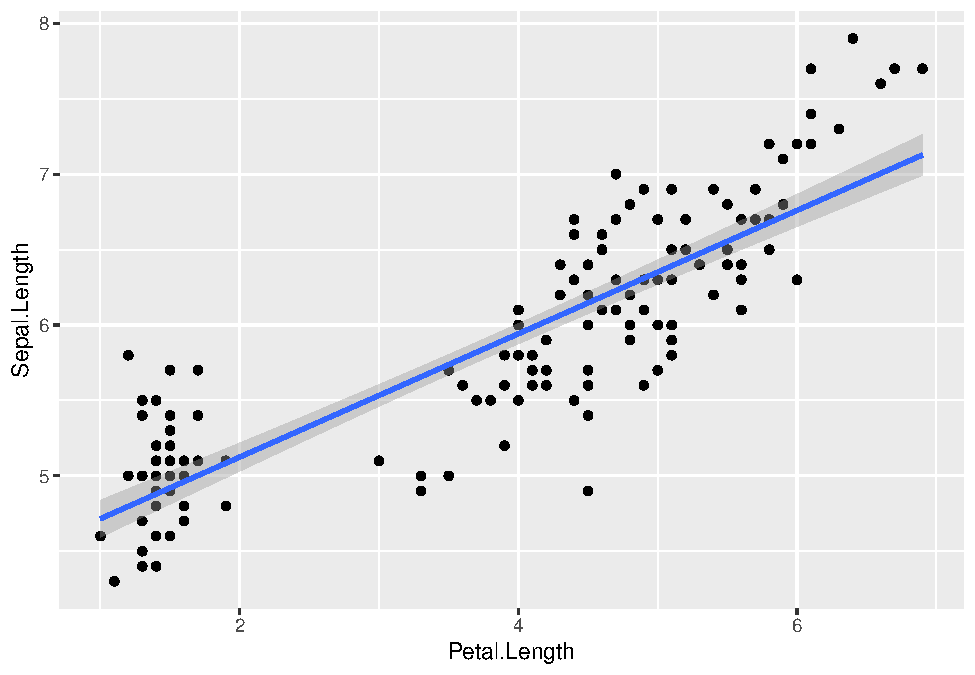
\includegraphics[width=1\linewidth]{paper_files/figure-latex/unnamed-chunk-5-1}

Now let's fit a Bayesian version of the model by using the
\texttt{stan\_glm} function in the \texttt{\{rstanarm\}} package:

\begin{Shaded}
\begin{Highlighting}[]
\NormalTok{model }\OtherTok{\textless{}{-}} \FunctionTok{stan\_glm}\NormalTok{(Sepal.Length }\SpecialCharTok{\textasciitilde{}}\NormalTok{ Petal.Length, }\AttributeTok{data =}\NormalTok{ iris)}
\CommentTok{\#\textgreater{} }
\CommentTok{\#\textgreater{} SAMPLING FOR MODEL \textquotesingle{}continuous\textquotesingle{} NOW (CHAIN 1).}
\CommentTok{\#\textgreater{} Chain 1: }
\CommentTok{\#\textgreater{} Chain 1: Gradient evaluation took 0.000266 seconds}
\CommentTok{\#\textgreater{} Chain 1: 1000 transitions using 10 leapfrog steps per transition would take 2.66 seconds.}
\CommentTok{\#\textgreater{} Chain 1: Adjust your expectations accordingly!}
\CommentTok{\#\textgreater{} Chain 1: }
\CommentTok{\#\textgreater{} Chain 1: }
\CommentTok{\#\textgreater{} Chain 1: Iteration:    1 / 2000 [  0\%]  (Warmup)}
\CommentTok{\#\textgreater{} Chain 1: Iteration:  200 / 2000 [ 10\%]  (Warmup)}
\CommentTok{\#\textgreater{} Chain 1: Iteration:  400 / 2000 [ 20\%]  (Warmup)}
\CommentTok{\#\textgreater{} Chain 1: Iteration:  600 / 2000 [ 30\%]  (Warmup)}
\CommentTok{\#\textgreater{} Chain 1: Iteration:  800 / 2000 [ 40\%]  (Warmup)}
\CommentTok{\#\textgreater{} Chain 1: Iteration: 1000 / 2000 [ 50\%]  (Warmup)}
\CommentTok{\#\textgreater{} Chain 1: Iteration: 1001 / 2000 [ 50\%]  (Sampling)}
\CommentTok{\#\textgreater{} Chain 1: Iteration: 1200 / 2000 [ 60\%]  (Sampling)}
\CommentTok{\#\textgreater{} Chain 1: Iteration: 1400 / 2000 [ 70\%]  (Sampling)}
\CommentTok{\#\textgreater{} Chain 1: Iteration: 1600 / 2000 [ 80\%]  (Sampling)}
\CommentTok{\#\textgreater{} Chain 1: Iteration: 1800 / 2000 [ 90\%]  (Sampling)}
\CommentTok{\#\textgreater{} Chain 1: Iteration: 2000 / 2000 [100\%]  (Sampling)}
\CommentTok{\#\textgreater{} Chain 1: }
\CommentTok{\#\textgreater{} Chain 1:  Elapsed Time: 0.024544 seconds (Warm{-}up)}
\CommentTok{\#\textgreater{} Chain 1:                0.035406 seconds (Sampling)}
\CommentTok{\#\textgreater{} Chain 1:                0.05995 seconds (Total)}
\CommentTok{\#\textgreater{} Chain 1: }
\CommentTok{\#\textgreater{} }
\CommentTok{\#\textgreater{} SAMPLING FOR MODEL \textquotesingle{}continuous\textquotesingle{} NOW (CHAIN 2).}
\CommentTok{\#\textgreater{} Chain 2: }
\CommentTok{\#\textgreater{} Chain 2: Gradient evaluation took 1.4e{-}05 seconds}
\CommentTok{\#\textgreater{} Chain 2: 1000 transitions using 10 leapfrog steps per transition would take 0.14 seconds.}
\CommentTok{\#\textgreater{} Chain 2: Adjust your expectations accordingly!}
\CommentTok{\#\textgreater{} Chain 2: }
\CommentTok{\#\textgreater{} Chain 2: }
\CommentTok{\#\textgreater{} Chain 2: Iteration:    1 / 2000 [  0\%]  (Warmup)}
\CommentTok{\#\textgreater{} Chain 2: Iteration:  200 / 2000 [ 10\%]  (Warmup)}
\CommentTok{\#\textgreater{} Chain 2: Iteration:  400 / 2000 [ 20\%]  (Warmup)}
\CommentTok{\#\textgreater{} Chain 2: Iteration:  600 / 2000 [ 30\%]  (Warmup)}
\CommentTok{\#\textgreater{} Chain 2: Iteration:  800 / 2000 [ 40\%]  (Warmup)}
\CommentTok{\#\textgreater{} Chain 2: Iteration: 1000 / 2000 [ 50\%]  (Warmup)}
\CommentTok{\#\textgreater{} Chain 2: Iteration: 1001 / 2000 [ 50\%]  (Sampling)}
\CommentTok{\#\textgreater{} Chain 2: Iteration: 1200 / 2000 [ 60\%]  (Sampling)}
\CommentTok{\#\textgreater{} Chain 2: Iteration: 1400 / 2000 [ 70\%]  (Sampling)}
\CommentTok{\#\textgreater{} Chain 2: Iteration: 1600 / 2000 [ 80\%]  (Sampling)}
\CommentTok{\#\textgreater{} Chain 2: Iteration: 1800 / 2000 [ 90\%]  (Sampling)}
\CommentTok{\#\textgreater{} Chain 2: Iteration: 2000 / 2000 [100\%]  (Sampling)}
\CommentTok{\#\textgreater{} Chain 2: }
\CommentTok{\#\textgreater{} Chain 2:  Elapsed Time: 0.024452 seconds (Warm{-}up)}
\CommentTok{\#\textgreater{} Chain 2:                0.033825 seconds (Sampling)}
\CommentTok{\#\textgreater{} Chain 2:                0.058277 seconds (Total)}
\CommentTok{\#\textgreater{} Chain 2: }
\CommentTok{\#\textgreater{} }
\CommentTok{\#\textgreater{} SAMPLING FOR MODEL \textquotesingle{}continuous\textquotesingle{} NOW (CHAIN 3).}
\CommentTok{\#\textgreater{} Chain 3: }
\CommentTok{\#\textgreater{} Chain 3: Gradient evaluation took 1.3e{-}05 seconds}
\CommentTok{\#\textgreater{} Chain 3: 1000 transitions using 10 leapfrog steps per transition would take 0.13 seconds.}
\CommentTok{\#\textgreater{} Chain 3: Adjust your expectations accordingly!}
\CommentTok{\#\textgreater{} Chain 3: }
\CommentTok{\#\textgreater{} Chain 3: }
\CommentTok{\#\textgreater{} Chain 3: Iteration:    1 / 2000 [  0\%]  (Warmup)}
\CommentTok{\#\textgreater{} Chain 3: Iteration:  200 / 2000 [ 10\%]  (Warmup)}
\CommentTok{\#\textgreater{} Chain 3: Iteration:  400 / 2000 [ 20\%]  (Warmup)}
\CommentTok{\#\textgreater{} Chain 3: Iteration:  600 / 2000 [ 30\%]  (Warmup)}
\CommentTok{\#\textgreater{} Chain 3: Iteration:  800 / 2000 [ 40\%]  (Warmup)}
\CommentTok{\#\textgreater{} Chain 3: Iteration: 1000 / 2000 [ 50\%]  (Warmup)}
\CommentTok{\#\textgreater{} Chain 3: Iteration: 1001 / 2000 [ 50\%]  (Sampling)}
\CommentTok{\#\textgreater{} Chain 3: Iteration: 1200 / 2000 [ 60\%]  (Sampling)}
\CommentTok{\#\textgreater{} Chain 3: Iteration: 1400 / 2000 [ 70\%]  (Sampling)}
\CommentTok{\#\textgreater{} Chain 3: Iteration: 1600 / 2000 [ 80\%]  (Sampling)}
\CommentTok{\#\textgreater{} Chain 3: Iteration: 1800 / 2000 [ 90\%]  (Sampling)}
\CommentTok{\#\textgreater{} Chain 3: Iteration: 2000 / 2000 [100\%]  (Sampling)}
\CommentTok{\#\textgreater{} Chain 3: }
\CommentTok{\#\textgreater{} Chain 3:  Elapsed Time: 0.029649 seconds (Warm{-}up)}
\CommentTok{\#\textgreater{} Chain 3:                0.047591 seconds (Sampling)}
\CommentTok{\#\textgreater{} Chain 3:                0.07724 seconds (Total)}
\CommentTok{\#\textgreater{} Chain 3: }
\CommentTok{\#\textgreater{} }
\CommentTok{\#\textgreater{} SAMPLING FOR MODEL \textquotesingle{}continuous\textquotesingle{} NOW (CHAIN 4).}
\CommentTok{\#\textgreater{} Chain 4: }
\CommentTok{\#\textgreater{} Chain 4: Gradient evaluation took 2.5e{-}05 seconds}
\CommentTok{\#\textgreater{} Chain 4: 1000 transitions using 10 leapfrog steps per transition would take 0.25 seconds.}
\CommentTok{\#\textgreater{} Chain 4: Adjust your expectations accordingly!}
\CommentTok{\#\textgreater{} Chain 4: }
\CommentTok{\#\textgreater{} Chain 4: }
\CommentTok{\#\textgreater{} Chain 4: Iteration:    1 / 2000 [  0\%]  (Warmup)}
\CommentTok{\#\textgreater{} Chain 4: Iteration:  200 / 2000 [ 10\%]  (Warmup)}
\CommentTok{\#\textgreater{} Chain 4: Iteration:  400 / 2000 [ 20\%]  (Warmup)}
\CommentTok{\#\textgreater{} Chain 4: Iteration:  600 / 2000 [ 30\%]  (Warmup)}
\CommentTok{\#\textgreater{} Chain 4: Iteration:  800 / 2000 [ 40\%]  (Warmup)}
\CommentTok{\#\textgreater{} Chain 4: Iteration: 1000 / 2000 [ 50\%]  (Warmup)}
\CommentTok{\#\textgreater{} Chain 4: Iteration: 1001 / 2000 [ 50\%]  (Sampling)}
\CommentTok{\#\textgreater{} Chain 4: Iteration: 1200 / 2000 [ 60\%]  (Sampling)}
\CommentTok{\#\textgreater{} Chain 4: Iteration: 1400 / 2000 [ 70\%]  (Sampling)}
\CommentTok{\#\textgreater{} Chain 4: Iteration: 1600 / 2000 [ 80\%]  (Sampling)}
\CommentTok{\#\textgreater{} Chain 4: Iteration: 1800 / 2000 [ 90\%]  (Sampling)}
\CommentTok{\#\textgreater{} Chain 4: Iteration: 2000 / 2000 [100\%]  (Sampling)}
\CommentTok{\#\textgreater{} Chain 4: }
\CommentTok{\#\textgreater{} Chain 4:  Elapsed Time: 0.034102 seconds (Warm{-}up)}
\CommentTok{\#\textgreater{} Chain 4:                0.048093 seconds (Sampling)}
\CommentTok{\#\textgreater{} Chain 4:                0.082195 seconds (Total)}
\CommentTok{\#\textgreater{} Chain 4:}
\end{Highlighting}
\end{Shaded}

You can see the sampling algorithm being run.

\hypertarget{extracting-the-posterior}{%
\subsubsection{Extracting the
posterior}\label{extracting-the-posterior}}

Once it is done, let us extract the parameters (\emph{i.e.},
coefficients) of the model.

\begin{Shaded}
\begin{Highlighting}[]
\NormalTok{posteriors }\OtherTok{\textless{}{-}}\NormalTok{ insight}\SpecialCharTok{::}\FunctionTok{get\_parameters}\NormalTok{(model)}

\FunctionTok{head}\NormalTok{(posteriors) }\CommentTok{\# Show the first 6 rows}
\CommentTok{\#\textgreater{}   (Intercept) Petal.Length}
\CommentTok{\#\textgreater{} 1    4.264526    0.4074007}
\CommentTok{\#\textgreater{} 2    4.294652    0.4052662}
\CommentTok{\#\textgreater{} 3    4.305143    0.4161953}
\CommentTok{\#\textgreater{} 4    4.392494    0.3946934}
\CommentTok{\#\textgreater{} 5    4.285853    0.4114136}
\CommentTok{\#\textgreater{} 6    4.381625    0.3923654}
\end{Highlighting}
\end{Shaded}

As we can see, the parameters take the form of a lengthy dataframe with
two columns, corresponding to the \texttt{intercept} and the effect of
\texttt{Petal.Length}. These columns contain the posterior distributions
of these two parameters. In simple terms, the posterior distribution is
a set of different plausible values for each parameter. Contrast this
with the result we saw from the frequentist linear regression mode using
\texttt{lm}, where the results had a single value for each effect of the
model, and not a distribution of values. This is one of the most
important differences between these two frameworks.

\hypertarget{posterior-draws}{%
\subsubsection{Posterior draws}\label{posterior-draws}}

Let's look at the length of the posteriors.

\begin{Shaded}
\begin{Highlighting}[]
\FunctionTok{nrow}\NormalTok{(posteriors) }\CommentTok{\# Size (number of rows)}
\CommentTok{\#\textgreater{} [1] 4000}
\end{Highlighting}
\end{Shaded}

Why is the size 4000, and not more or less?

First of all, these observations (the rows) are usually referred to as
\emph{posterior draws}. The underlying idea is that the Bayesian
sampling algorithm (\emph{e.g.}, Monte Carlo Markov Chains - MCMC) will
\emph{draw} from the hidden true posterior distribution. Thus, it is
through these posterior draws that we can estimate the underlying true
posterior distribution. Therefore, the more draws you have, the better
your estimation of the posterior distribution. However, increased draws
also means longer computation time.

If we look at the documentation (\texttt{?sampling}) for the
\texttt{rstanarm}'s \texttt{"sampling"} algorithm used by default in the
model above, we can see several parameters that influence the number of
posterior draws. By default, there are 4 \texttt{chains} (you can see it
as distinct sampling runs), that each create 2000 \texttt{iter} (draws).
However, only half of these iterations are kept, as half are used for
\texttt{warm-up} (the convergence of the algorithm). Thus, the total for
posterior draws equals
\texttt{4\ chains\ *\ (2000\ iterations\ -\ 1000\ warm-up)\ =\ 4000}.

We can change that, for instance:

\begin{Shaded}
\begin{Highlighting}[]
\NormalTok{model }\OtherTok{\textless{}{-}} \FunctionTok{stan\_glm}\NormalTok{(}
    \AttributeTok{formula =}\NormalTok{ Sepal.Length }\SpecialCharTok{\textasciitilde{}}\NormalTok{ Petal.Length,}
    \AttributeTok{data =}\NormalTok{ iris,}
    \AttributeTok{chains =} \DecValTok{2}\NormalTok{,}
    \AttributeTok{iter =} \DecValTok{1000}\NormalTok{,}
    \AttributeTok{warmup =} \DecValTok{250}
\NormalTok{  )}
\CommentTok{\#\textgreater{} }
\CommentTok{\#\textgreater{} SAMPLING FOR MODEL \textquotesingle{}continuous\textquotesingle{} NOW (CHAIN 1).}
\CommentTok{\#\textgreater{} Chain 1: }
\CommentTok{\#\textgreater{} Chain 1: Gradient evaluation took 2.1e{-}05 seconds}
\CommentTok{\#\textgreater{} Chain 1: 1000 transitions using 10 leapfrog steps per transition would take 0.21 seconds.}
\CommentTok{\#\textgreater{} Chain 1: Adjust your expectations accordingly!}
\CommentTok{\#\textgreater{} Chain 1: }
\CommentTok{\#\textgreater{} Chain 1: }
\CommentTok{\#\textgreater{} Chain 1: Iteration:   1 / 1000 [  0\%]  (Warmup)}
\CommentTok{\#\textgreater{} Chain 1: Iteration: 100 / 1000 [ 10\%]  (Warmup)}
\CommentTok{\#\textgreater{} Chain 1: Iteration: 200 / 1000 [ 20\%]  (Warmup)}
\CommentTok{\#\textgreater{} Chain 1: Iteration: 251 / 1000 [ 25\%]  (Sampling)}
\CommentTok{\#\textgreater{} Chain 1: Iteration: 350 / 1000 [ 35\%]  (Sampling)}
\CommentTok{\#\textgreater{} Chain 1: Iteration: 450 / 1000 [ 45\%]  (Sampling)}
\CommentTok{\#\textgreater{} Chain 1: Iteration: 550 / 1000 [ 55\%]  (Sampling)}
\CommentTok{\#\textgreater{} Chain 1: Iteration: 650 / 1000 [ 65\%]  (Sampling)}
\CommentTok{\#\textgreater{} Chain 1: Iteration: 750 / 1000 [ 75\%]  (Sampling)}
\CommentTok{\#\textgreater{} Chain 1: Iteration: 850 / 1000 [ 85\%]  (Sampling)}
\CommentTok{\#\textgreater{} Chain 1: Iteration: 950 / 1000 [ 95\%]  (Sampling)}
\CommentTok{\#\textgreater{} Chain 1: Iteration: 1000 / 1000 [100\%]  (Sampling)}
\CommentTok{\#\textgreater{} Chain 1: }
\CommentTok{\#\textgreater{} Chain 1:  Elapsed Time: 0.011527 seconds (Warm{-}up)}
\CommentTok{\#\textgreater{} Chain 1:                0.037453 seconds (Sampling)}
\CommentTok{\#\textgreater{} Chain 1:                0.04898 seconds (Total)}
\CommentTok{\#\textgreater{} Chain 1: }
\CommentTok{\#\textgreater{} }
\CommentTok{\#\textgreater{} SAMPLING FOR MODEL \textquotesingle{}continuous\textquotesingle{} NOW (CHAIN 2).}
\CommentTok{\#\textgreater{} Chain 2: }
\CommentTok{\#\textgreater{} Chain 2: Gradient evaluation took 2.3e{-}05 seconds}
\CommentTok{\#\textgreater{} Chain 2: 1000 transitions using 10 leapfrog steps per transition would take 0.23 seconds.}
\CommentTok{\#\textgreater{} Chain 2: Adjust your expectations accordingly!}
\CommentTok{\#\textgreater{} Chain 2: }
\CommentTok{\#\textgreater{} Chain 2: }
\CommentTok{\#\textgreater{} Chain 2: Iteration:   1 / 1000 [  0\%]  (Warmup)}
\CommentTok{\#\textgreater{} Chain 2: Iteration: 100 / 1000 [ 10\%]  (Warmup)}
\CommentTok{\#\textgreater{} Chain 2: Iteration: 200 / 1000 [ 20\%]  (Warmup)}
\CommentTok{\#\textgreater{} Chain 2: Iteration: 251 / 1000 [ 25\%]  (Sampling)}
\CommentTok{\#\textgreater{} Chain 2: Iteration: 350 / 1000 [ 35\%]  (Sampling)}
\CommentTok{\#\textgreater{} Chain 2: Iteration: 450 / 1000 [ 45\%]  (Sampling)}
\CommentTok{\#\textgreater{} Chain 2: Iteration: 550 / 1000 [ 55\%]  (Sampling)}
\CommentTok{\#\textgreater{} Chain 2: Iteration: 650 / 1000 [ 65\%]  (Sampling)}
\CommentTok{\#\textgreater{} Chain 2: Iteration: 750 / 1000 [ 75\%]  (Sampling)}
\CommentTok{\#\textgreater{} Chain 2: Iteration: 850 / 1000 [ 85\%]  (Sampling)}
\CommentTok{\#\textgreater{} Chain 2: Iteration: 950 / 1000 [ 95\%]  (Sampling)}
\CommentTok{\#\textgreater{} Chain 2: Iteration: 1000 / 1000 [100\%]  (Sampling)}
\CommentTok{\#\textgreater{} Chain 2: }
\CommentTok{\#\textgreater{} Chain 2:  Elapsed Time: 0.011218 seconds (Warm{-}up)}
\CommentTok{\#\textgreater{} Chain 2:                0.038522 seconds (Sampling)}
\CommentTok{\#\textgreater{} Chain 2:                0.04974 seconds (Total)}
\CommentTok{\#\textgreater{} Chain 2:}

\FunctionTok{nrow}\NormalTok{(insight}\SpecialCharTok{::}\FunctionTok{get\_parameters}\NormalTok{(model)) }\CommentTok{\# Size (number of rows)}
\CommentTok{\#\textgreater{} [1] 1500}
\end{Highlighting}
\end{Shaded}

In this case, as would be expected, we have
\texttt{2\ chains\ *\ (1000\ iterations\ -\ 250\ warm-up)\ =\ 1500}
posterior draws. But let's keep our first model with the default setup
(as it has more draws).

\hypertarget{visualizing-the-posterior-distribution}{%
\paragraph{Visualizing the posterior
distribution}\label{visualizing-the-posterior-distribution}}

Now that we've understood where these values come from, let's look at
them. We will start by visualizing the posterior distribution of our
parameter of interest, the effect of \texttt{Petal.Length}.

\begin{Shaded}
\begin{Highlighting}[]
\FunctionTok{ggplot}\NormalTok{(posteriors, }\FunctionTok{aes}\NormalTok{(}\AttributeTok{x =}\NormalTok{ Petal.Length)) }\SpecialCharTok{+}
  \FunctionTok{geom\_density}\NormalTok{(}\AttributeTok{fill =} \StringTok{"orange"}\NormalTok{)}
\end{Highlighting}
\end{Shaded}

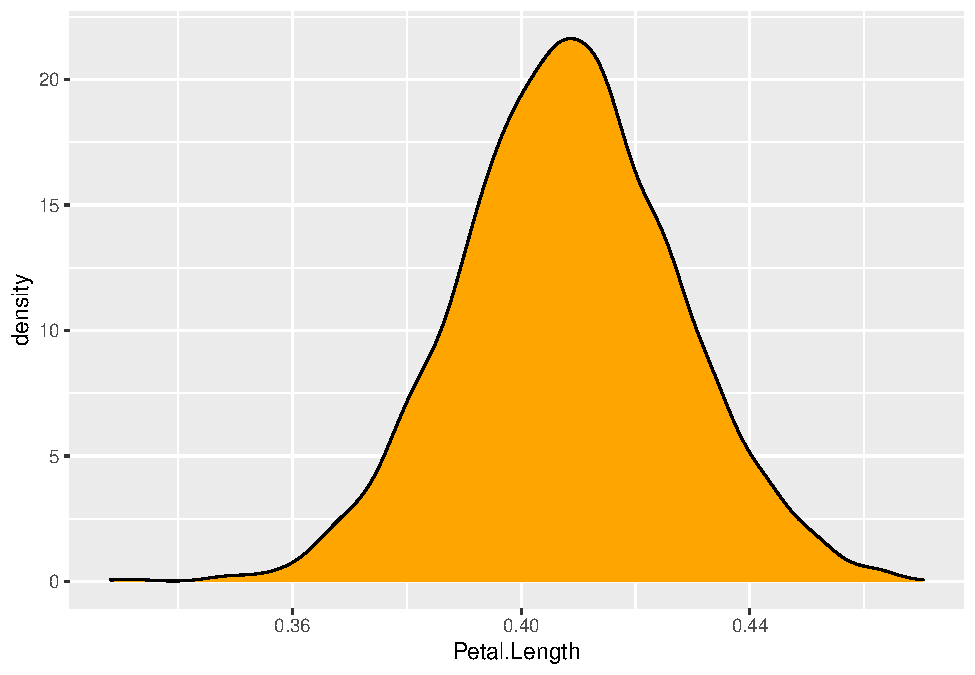
\includegraphics[width=1\linewidth]{paper_files/figure-latex/unnamed-chunk-10-1}

This distribution represents the
\href{https://en.wikipedia.org/wiki/Probability_density_function}{probability}
(the \texttt{y} axis) of different effects (the \texttt{x} axis). The
central values are more probable than the extreme values. As you can
see, this distribution ranges from about 0.35 to 0.50, with the bulk of
it being at around 0.41. This is it, we've just described your first
posterior distribution.

And this is the heart of Bayesian analysis. We don't need
\emph{p}-values, \emph{t}-values, or degrees of freedom. Everything we
need is contained within this posterior distribution.

Our description above is consistent with the values obtained from the
frequentist regression (which resulted in a \(\beta\) of 0.41). This is
reassuring! Indeed, in most cases, Bayesian analysis does not
drastically differ from the frequentist results or their interpretation.
Rather, it makes the results more interpretable and intuitive, and
easier to understand and describe. We can now go ahead and precisely
characterize this posterior distribution.

\hypertarget{describing-the-posterior}{%
\subsubsection{Describing the
Posterior}\label{describing-the-posterior}}

Unfortunately, it is often not practical to report the whole posterior
distributions as graphs. We need to find a concise way to summarize it.
We recommend to describe the posterior distribution with 3 elements:

\begin{enumerate}
\def\labelenumi{\arabic{enumi}.}
\tightlist
\item
  A point-estimate which is a one-value summary (similar to the \(beta\)
  in frequentist regressions).
\item
  A credible interval representing the associated uncertainty.
\item
  Some indices of significance, giving information about the relative
  importance of this effect.
\end{enumerate}

\hypertarget{point-estimate}{%
\paragraph{Point-estimate}\label{point-estimate}}

What single value can best represent my posterior distribution?

Centrality indices, such as the \emph{mean}, the \emph{median}, or the
\emph{mode} are usually used as point-estimates. But what's the
difference between them?

Let's answer this by first inspecting the mean:

\begin{Shaded}
\begin{Highlighting}[]
\FunctionTok{mean}\NormalTok{(posteriors}\SpecialCharTok{$}\NormalTok{Petal.Length)}
\CommentTok{\#\textgreater{} [1] 0.4081661}
\end{Highlighting}
\end{Shaded}

This is close to the frequentist \(\beta\). But, as we know, the mean is
quite sensitive to outliers or extremes values. Maybe the median could
be more robust?

\begin{Shaded}
\begin{Highlighting}[]
\FunctionTok{median}\NormalTok{(posteriors}\SpecialCharTok{$}\NormalTok{Petal.Length)}
\CommentTok{\#\textgreater{} [1] 0.4079311}
\end{Highlighting}
\end{Shaded}

Well, this is very close to the mean (and identical when rounding the
values). Maybe we could take the mode, that is, the \emph{peak} of the
posterior distribution? In the Bayesian framework, this value is called
the Maximum A Posteriori (MAP). Let's see:

\begin{Shaded}
\begin{Highlighting}[]
\FunctionTok{map\_estimate}\NormalTok{(posteriors}\SpecialCharTok{$}\NormalTok{Petal.Length)}
\CommentTok{\#\textgreater{} MAP Estimate: 0.41}
\end{Highlighting}
\end{Shaded}

They are all very close!

Let's visualize these values on the posterior distribution:

\begin{Shaded}
\begin{Highlighting}[]
\FunctionTok{ggplot}\NormalTok{(posteriors, }\FunctionTok{aes}\NormalTok{(}\AttributeTok{x =}\NormalTok{ Petal.Length)) }\SpecialCharTok{+}
  \FunctionTok{geom\_density}\NormalTok{(}\AttributeTok{fill =} \StringTok{"orange"}\NormalTok{) }\SpecialCharTok{+}
  \CommentTok{\# The mean in blue}
  \FunctionTok{geom\_vline}\NormalTok{(}\AttributeTok{xintercept =} \FunctionTok{mean}\NormalTok{(posteriors}\SpecialCharTok{$}\NormalTok{Petal.Length), }\AttributeTok{color =} \StringTok{"blue"}\NormalTok{, }\AttributeTok{size =} \DecValTok{1}\NormalTok{) }\SpecialCharTok{+}
  \CommentTok{\# The median in red}
  \FunctionTok{geom\_vline}\NormalTok{(}\AttributeTok{xintercept =} \FunctionTok{median}\NormalTok{(posteriors}\SpecialCharTok{$}\NormalTok{Petal.Length), }\AttributeTok{color =} \StringTok{"red"}\NormalTok{, }\AttributeTok{size =} \DecValTok{1}\NormalTok{) }\SpecialCharTok{+}
  \CommentTok{\# The MAP in purple}
  \FunctionTok{geom\_vline}\NormalTok{(}\AttributeTok{xintercept =} \FunctionTok{map\_estimate}\NormalTok{(posteriors}\SpecialCharTok{$}\NormalTok{Petal.Length), }\AttributeTok{color =} \StringTok{"purple"}\NormalTok{, }\AttributeTok{size =} \DecValTok{1}\NormalTok{)}
\end{Highlighting}
\end{Shaded}

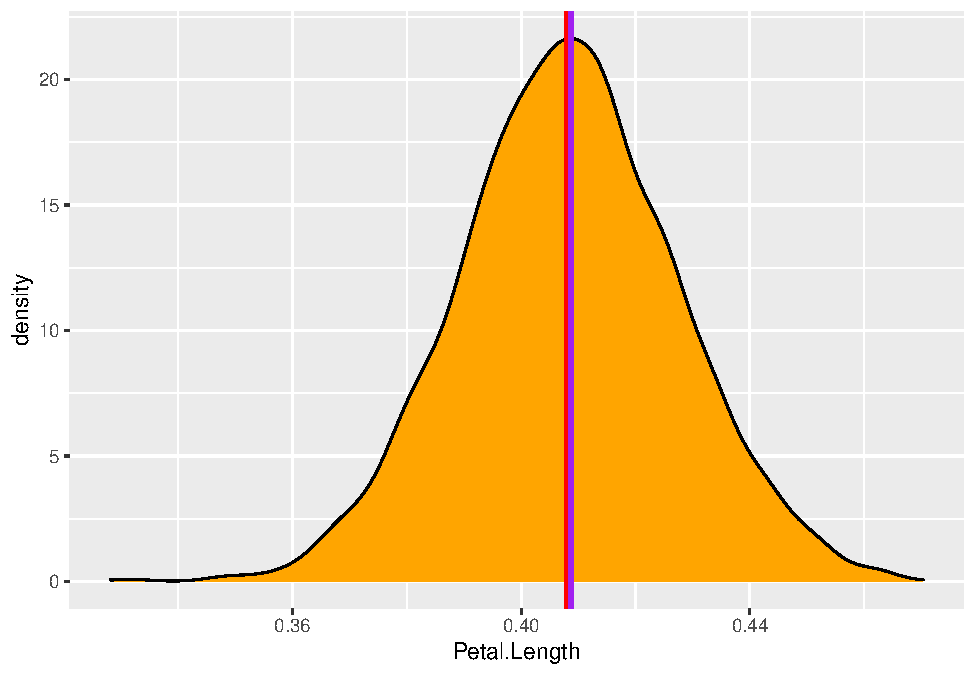
\includegraphics[width=1\linewidth]{paper_files/figure-latex/unnamed-chunk-14-1}

Well, all these values give very similar results. Thus, we will choose
the median, as this value has a direct meaning from a probabilistic
perspective: there is 50\% chance that the true effect is higher and
50\% chance that the effect is lower (as it divides the distribution in
two equal parts).

\hypertarget{uncertainty}{%
\paragraph{Uncertainty}\label{uncertainty}}

Now that the have a point-estimate, we have to describe the uncertainty.
We could compute the range:

\begin{Shaded}
\begin{Highlighting}[]
\FunctionTok{range}\NormalTok{(posteriors}\SpecialCharTok{$}\NormalTok{Petal.Length)}
\CommentTok{\#\textgreater{} [1] 0.3281408 0.4702873}
\end{Highlighting}
\end{Shaded}

But does it make sense to include all these extreme values? Probably
not. Thus, we will compute a
\href{https://easystats.github.io/bayestestR/articles/credible_interval.html}{credible
interval}. Long story short, it's kind of similar to a frequentist
confidence interval, but easier to interpret and easier to compute ---
and it makes more sense.

We will compute this credible interval based on the Highest Density
Interval (HDI). It will give us the range containing the 89\% most
probable effect values. Note that we will use 89\% CIs instead of 95\%
CIs (as in the frequentist framework), as the 89\% level gives more
stable results (\protect\hyperlink{ref-kruschke2014doing}{J. Kruschke,
2014}) and reminds us about the arbitrariness of such conventions
(\protect\hyperlink{ref-mcelreath2018statistical}{McElreath, 2018}).

\begin{Shaded}
\begin{Highlighting}[]
\FunctionTok{hdi}\NormalTok{(posteriors}\SpecialCharTok{$}\NormalTok{Petal.Length, }\AttributeTok{ci =} \FloatTok{0.89}\NormalTok{)}
\CommentTok{\#\textgreater{} 89\% HDI: [0.38, 0.44]}
\end{Highlighting}
\end{Shaded}

Nice, so we can conclude that the effect has 89\% chance of falling
within the \texttt{{[}0.38,\ 0.44{]}} range. We have just computed the
two most important pieces of information for describing our effects.

\hypertarget{effect-significance}{%
\paragraph{Effect significance}\label{effect-significance}}

However, in many scientific fields it not sufficient to simply describe
the effects. Scientists also want to know if this effect has
significance in practical or statistical terms, or in other words,
whether the effect is important. For instance, is the effect different
from 0? So how do we assess the \emph{significance} of an effect. How
can we do this?

Well, in this particular case, it is very eloquent: all possible effect
values (\emph{i.e.}, the whole posterior distribution) are positive and
over 0.35, which is already substantial evidence the effect is not zero.

But still, we want some objective decision criterion, to say if yes or
no the effect is `significant.' One approach, similar to the frequentist
framework, would be to see if the Credible Interval contains 0. If it is
not the case, that would mean that our effect is `significant.'

But this index is not very fine-grained, no? Can we do better? Yes!

\hypertarget{a-linear-model-with-a-categorical-predictor}{%
\subsection{A linear model with a categorical
predictor}\label{a-linear-model-with-a-categorical-predictor}}

Imagine for a moment you are interested in how the weight of chickens
varies depending on two different feed types. For this example, we will
start by selecting from the \texttt{chickwts} dataset (available in base
R) two feed types of interest for us (\emph{we do have peculiar
interests}): meat meals and sunflowers.

\hypertarget{data-preparation-and-model-fitting}{%
\subsubsection{Data preparation and model
fitting}\label{data-preparation-and-model-fitting}}

\begin{Shaded}
\begin{Highlighting}[]
\FunctionTok{library}\NormalTok{(dplyr)}

\CommentTok{\# We keep only rows for which feed is meatmeal or sunflower}
\NormalTok{data }\OtherTok{\textless{}{-}} \FunctionTok{filter}\NormalTok{(chickwts, feed }\SpecialCharTok{\%in\%} \FunctionTok{c}\NormalTok{(}\StringTok{"meatmeal"}\NormalTok{, }\StringTok{"sunflower"}\NormalTok{))}
\end{Highlighting}
\end{Shaded}

Let's run another Bayesian regression to predict the weight with the two
types of feed type.

\begin{Shaded}
\begin{Highlighting}[]
\NormalTok{model }\OtherTok{\textless{}{-}} \FunctionTok{stan\_glm}\NormalTok{(weight }\SpecialCharTok{\textasciitilde{}}\NormalTok{ feed, }\AttributeTok{data =}\NormalTok{ data)}
\end{Highlighting}
\end{Shaded}

\hypertarget{posterior-description}{%
\subsubsection{Posterior description}\label{posterior-description}}

\begin{Shaded}
\begin{Highlighting}[]
\NormalTok{posteriors }\OtherTok{\textless{}{-}}\NormalTok{ insight}\SpecialCharTok{::}\FunctionTok{get\_parameters}\NormalTok{(model)}

\FunctionTok{ggplot}\NormalTok{(posteriors, }\FunctionTok{aes}\NormalTok{(}\AttributeTok{x =}\NormalTok{ feedsunflower)) }\SpecialCharTok{+}
  \FunctionTok{geom\_density}\NormalTok{(}\AttributeTok{fill =} \StringTok{"red"}\NormalTok{)}
\end{Highlighting}
\end{Shaded}

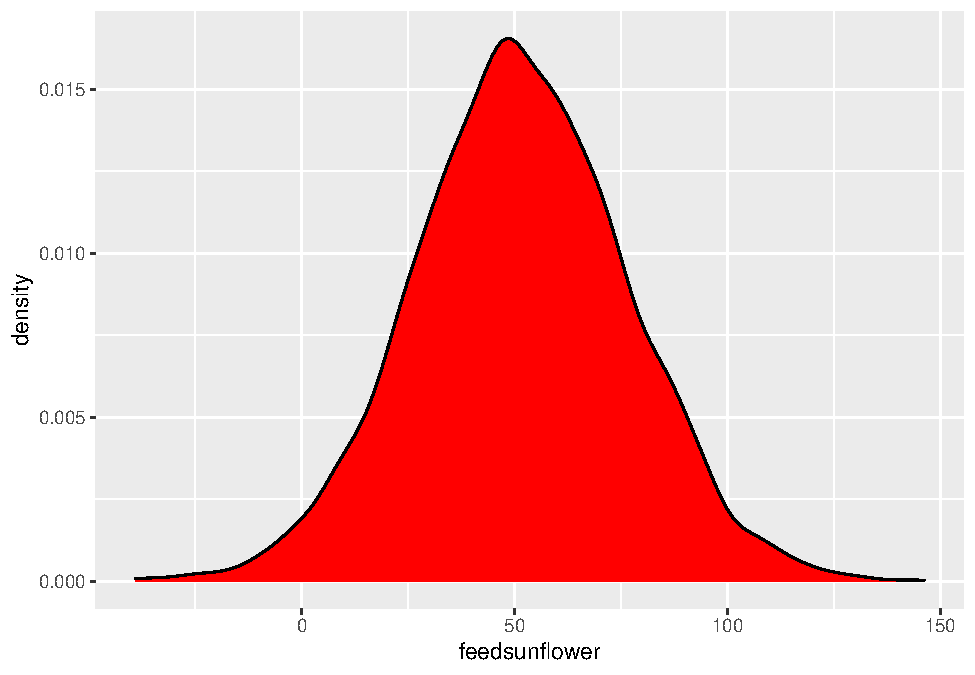
\includegraphics[width=1\linewidth]{paper_files/figure-latex/unnamed-chunk-20-1}

This represents the posterior distribution of the difference between
\texttt{meatmeal} and \texttt{sunflowers}. It seems that the difference
is positive (since the values are concentrated on the right side of 0).
Eating sunflowers makes you more fat (\emph{at least, if you're a
chicken}). But, by how much?

Let us compute the median and the CI:

\begin{Shaded}
\begin{Highlighting}[]
\FunctionTok{median}\NormalTok{(posteriors}\SpecialCharTok{$}\NormalTok{feedsunflower)}
\CommentTok{\#\textgreater{} [1] 50.84833}
\FunctionTok{hdi}\NormalTok{(posteriors}\SpecialCharTok{$}\NormalTok{feedsunflower)}
\CommentTok{\#\textgreater{} 95\% HDI: [0.74, 98.31]}
\end{Highlighting}
\end{Shaded}

It makes you fat by around 51 grams (the median). However, the
uncertainty is quite high: there is 89\% chance that the difference
between the two feed types is between 14 and 91. Is this effect
different from 0?

\hypertarget{rope-percentage}{%
\subsubsection{ROPE Percentage}\label{rope-percentage}}

Testing whether this distribution is different from 0 doesn't make
sense, as 0 is a single value (and the probability that any distribution
is different from a single value is infinite).

However, one way to assess significance could be to define an area
\emph{around} 0, which will consider as \emph{practically equivalent} to
zero (\emph{i.e.}, absence of, or a negligible, effect). This is called
the Region of Practical Equivalence (ROPE), and is one way of testing
the significance of parameters.

How can we define this region? We know that we can define the ROPE as
the \texttt{{[}-20,\ 20{]}} range. All effects within this range are
considered as \emph{null} (negligible). We can now compute the
proportion of the 89\% most probable values (the 89\% CI) which are not
null, \emph{i.e.}, which are outside this range.

\begin{Shaded}
\begin{Highlighting}[]
\FunctionTok{rope}\NormalTok{(posteriors}\SpecialCharTok{$}\NormalTok{feedsunflower, }\AttributeTok{range =} \FunctionTok{c}\NormalTok{(}\SpecialCharTok{{-}}\DecValTok{20}\NormalTok{, }\DecValTok{20}\NormalTok{), }\AttributeTok{ci =} \FloatTok{0.89}\NormalTok{)}
\CommentTok{\#\textgreater{} \# Proportion of samples inside the ROPE [{-}20.00, 20.00]:}
\CommentTok{\#\textgreater{} }
\CommentTok{\#\textgreater{} inside ROPE}
\CommentTok{\#\textgreater{} {-}{-}{-}{-}{-}{-}{-}{-}{-}{-}{-}}
\CommentTok{\#\textgreater{} 4.86 \%}
\end{Highlighting}
\end{Shaded}

5\% of the 89\% CI can be considered as null. Is that a lot? Based on
our
\href{https://easystats.github.io/bayestestR/articles/guidelines.html}{guidelines},
yes, it is too much. Based on this particular definition of ROPE, we
conclude that this effect is not significant (the probability of being
negligible is too high).

That said, to be honest, I have some doubts about this Prof.~Sanders. I
don't really trust his definition of ROPE. Is there a more objective way
of defining it?

Yes! One of the practice is for instance to use the tenth
(\texttt{1/10\ =\ 0.1}) of the standard deviation (SD) of the response
variable, which can be considered as a ``negligible'' effect size
(\protect\hyperlink{ref-cohen1988statistical}{Cohen, 1988}).

\begin{Shaded}
\begin{Highlighting}[]
\NormalTok{rope\_value }\OtherTok{\textless{}{-}} \FloatTok{0.1} \SpecialCharTok{*} \FunctionTok{sd}\NormalTok{(data}\SpecialCharTok{$}\NormalTok{weight)}
\NormalTok{rope\_range }\OtherTok{\textless{}{-}} \FunctionTok{c}\NormalTok{(}\SpecialCharTok{{-}}\NormalTok{rope\_value, rope\_value)}
\NormalTok{rope\_range}
\CommentTok{\#\textgreater{} [1] {-}6.17469  6.17469}
\end{Highlighting}
\end{Shaded}

Let's redefine our ROPE as the region within the
\texttt{{[}-6.2,\ 6.2{]}} range. Note that this can be directly obtained
by the \texttt{rope\_range} function :)

\begin{Shaded}
\begin{Highlighting}[]
\NormalTok{rope\_value }\OtherTok{\textless{}{-}} \FunctionTok{rope\_range}\NormalTok{(model)}
\NormalTok{rope\_value}
\CommentTok{\#\textgreater{} [1] {-}6.17469  6.17469}
\end{Highlighting}
\end{Shaded}

Let's recompute the percentage in ROPE:

\begin{Shaded}
\begin{Highlighting}[]
\FunctionTok{rope}\NormalTok{(posteriors}\SpecialCharTok{$}\NormalTok{feedsunflower, }\AttributeTok{range =}\NormalTok{ rope\_range, }\AttributeTok{ci =} \FloatTok{0.89}\NormalTok{)}
\CommentTok{\#\textgreater{} \# Proportion of samples inside the ROPE [{-}6.17, 6.17]:}
\CommentTok{\#\textgreater{} }
\CommentTok{\#\textgreater{} inside ROPE}
\CommentTok{\#\textgreater{} {-}{-}{-}{-}{-}{-}{-}{-}{-}{-}{-}}
\CommentTok{\#\textgreater{} 0.00 \%}
\end{Highlighting}
\end{Shaded}

With this reasonable definition of ROPE, we observe that the 89\% of the
posterior distribution of the effect does not overlap with the ROPE.
Thus, we can conclude that the effect is significant (in the sense of
\emph{important} enough to be noted).

\hypertarget{probability-of-direction-pd}{%
\subsubsection{Probability of Direction
(pd)}\label{probability-of-direction-pd}}

Maybe we are not interested in whether the effect is non-negligible.
Maybe we just want to know if this effect is positive or negative. In
this case, we can simply compute the proportion of the posterior that is
positive, no matter the ``size'' of the effect.

\begin{Shaded}
\begin{Highlighting}[]
\NormalTok{n\_positive }\OtherTok{\textless{}{-}}\NormalTok{ posteriors }\SpecialCharTok{\%\textgreater{}\%}
  \FunctionTok{filter}\NormalTok{(feedsunflower }\SpecialCharTok{\textgreater{}} \DecValTok{0}\NormalTok{) }\SpecialCharTok{\%\textgreater{}\%} \CommentTok{\# select only positive values}
  \FunctionTok{nrow}\NormalTok{() }\CommentTok{\# Get length}

\NormalTok{n\_positive }\SpecialCharTok{/} \FunctionTok{nrow}\NormalTok{(posteriors) }\SpecialCharTok{*} \DecValTok{100}
\CommentTok{\#\textgreater{} [1] 97.925}
\end{Highlighting}
\end{Shaded}

We can conclude that the effect is positive with a probability of 98\%.
We call this index the Probability of Direction (pd). It can, in fact,
be computed more easily with the following:

\begin{Shaded}
\begin{Highlighting}[]
\FunctionTok{p\_direction}\NormalTok{(posteriors}\SpecialCharTok{$}\NormalTok{feedsunflower)}
\CommentTok{\#\textgreater{} Probability of Direction: 0.98}
\end{Highlighting}
\end{Shaded}

Interestingly, it so happens that this index is usually highly
correlated with the frequentist \emph{p}-value. We could almost roughly
infer the corresponding \emph{p}-value with a simple transformation:

\begin{Shaded}
\begin{Highlighting}[]
\NormalTok{pd }\OtherTok{\textless{}{-}} \FloatTok{97.82}
\NormalTok{onesided\_p }\OtherTok{\textless{}{-}} \DecValTok{1} \SpecialCharTok{{-}}\NormalTok{ pd }\SpecialCharTok{/} \DecValTok{100}
\NormalTok{twosided\_p }\OtherTok{\textless{}{-}}\NormalTok{ onesided\_p }\SpecialCharTok{*} \DecValTok{2}
\NormalTok{twosided\_p}
\CommentTok{\#\textgreater{} [1] 0.0436}
\end{Highlighting}
\end{Shaded}

If we ran our model in the frequentist framework, we should
approximately observe an effect with a \emph{p}-value of 0.044. Is that
true?

\hypertarget{comparison-to-frequentist}{%
\paragraph{Comparison to frequentist}\label{comparison-to-frequentist}}

\begin{Shaded}
\begin{Highlighting}[]
\FunctionTok{summary}\NormalTok{(}\FunctionTok{lm}\NormalTok{(weight }\SpecialCharTok{\textasciitilde{}}\NormalTok{ feed, }\AttributeTok{data =}\NormalTok{ data))}
\CommentTok{\#\textgreater{} }
\CommentTok{\#\textgreater{} Call:}
\CommentTok{\#\textgreater{} lm(formula = weight \textasciitilde{} feed, data = data)}
\CommentTok{\#\textgreater{} }
\CommentTok{\#\textgreater{} Residuals:}
\CommentTok{\#\textgreater{}      Min       1Q   Median       3Q      Max }
\CommentTok{\#\textgreater{} {-}123.909  {-}25.913   {-}6.917   32.091  103.091 }
\CommentTok{\#\textgreater{} }
\CommentTok{\#\textgreater{} Coefficients:}
\CommentTok{\#\textgreater{}               Estimate Std. Error t value Pr(\textgreater{}|t|)    }
\CommentTok{\#\textgreater{} (Intercept)     276.91      17.20  16.097 2.74e{-}13 ***}
\CommentTok{\#\textgreater{} feedsunflower    52.01      23.82   2.184   0.0405 *  }
\CommentTok{\#\textgreater{} {-}{-}{-}}
\CommentTok{\#\textgreater{} Signif. codes:  0 \textquotesingle{}***\textquotesingle{} 0.001 \textquotesingle{}**\textquotesingle{} 0.01 \textquotesingle{}*\textquotesingle{} 0.05 \textquotesingle{}.\textquotesingle{} 0.1 \textquotesingle{} \textquotesingle{} 1}
\CommentTok{\#\textgreater{} }
\CommentTok{\#\textgreater{} Residual standard error: 57.05 on 21 degrees of freedom}
\CommentTok{\#\textgreater{} Multiple R{-}squared:  0.1851, Adjusted R{-}squared:  0.1463 }
\CommentTok{\#\textgreater{} F{-}statistic: 4.769 on 1 and 21 DF,  p{-}value: 0.04047}
\end{Highlighting}
\end{Shaded}

The frequentist model tells us that the difference is positive and
significant (\(\beta = 52, p = 0.04\)).

Although we arrived to a similar conclusion, the Bayesian framework
allowed us to develop a more profound and intuitive understanding of our
effect, and of the uncertainty of its estimation.

\hypertarget{all-with-one-function}{%
\subsection{All with one function}\label{all-with-one-function}}

And yet, I agree, it was a bit tedious to extract and compute all the
indices. But what if I told you that we can do all of this, and more,
with only one function? Behold, \texttt{describe\_posterior}!

This function computes all of the adored mentioned indices, and can be
run directly on the model:

\begin{Shaded}
\begin{Highlighting}[]
\FunctionTok{describe\_posterior}\NormalTok{(model, }\AttributeTok{test =} \FunctionTok{c}\NormalTok{(}\StringTok{"p\_direction"}\NormalTok{, }\StringTok{"rope"}\NormalTok{, }\StringTok{"bayesfactor"}\NormalTok{))}
\CommentTok{\#\textgreater{} Summary of Posterior Distribution}
\CommentTok{\#\textgreater{} }
\CommentTok{\#\textgreater{} Parameter     | Median |           95\% CI |     pd |          ROPE | \% in ROPE |  Rhat |     ESS |     BF}
\CommentTok{\#\textgreater{} {-}{-}{-}{-}{-}{-}{-}{-}{-}{-}{-}{-}{-}{-}{-}{-}{-}{-}{-}{-}{-}{-}{-}{-}{-}{-}{-}{-}{-}{-}{-}{-}{-}{-}{-}{-}{-}{-}{-}{-}{-}{-}{-}{-}{-}{-}{-}{-}{-}{-}{-}{-}{-}{-}{-}{-}{-}{-}{-}{-}{-}{-}{-}{-}{-}{-}{-}{-}{-}{-}{-}{-}{-}{-}{-}{-}{-}{-}{-}{-}{-}{-}{-}{-}{-}{-}{-}{-}{-}{-}{-}{-}{-}{-}{-}{-}{-}{-}{-}{-}{-}{-}{-}{-}{-}}
\CommentTok{\#\textgreater{} (Intercept)   | 277.27 | [240.57, 313.01] |   100\% | [{-}6.17, 6.17] |        0\% | 1.000 | 3678.00 | \textgreater{} 1000}
\CommentTok{\#\textgreater{} feedsunflower |  50.85 | [  0.74,  98.31] | 97.92\% | [{-}6.17, 6.17] |     1.26\% | 1.001 | 3723.00 |  0.727}
\end{Highlighting}
\end{Shaded}

There we have it! The median, the CI, the pd and the ROPE percentage.

\hypertarget{correlations}{%
\subsection{Correlations}\label{correlations}}

\hypertarget{frequentist-version}{%
\subsubsection{Frequentist version}\label{frequentist-version}}

Once again, let us begin with a frequentist correlation between two
continuous variables, the width and the length of the sepals of some
flowers. The data is available in \texttt{R} as the \texttt{iris}
dataset.

We will compute a Pearson's correlation test, store the results in an
object called \texttt{result}, and then display it:

\begin{Shaded}
\begin{Highlighting}[]
\NormalTok{result }\OtherTok{\textless{}{-}} \FunctionTok{cor.test}\NormalTok{(iris}\SpecialCharTok{$}\NormalTok{Sepal.Width, iris}\SpecialCharTok{$}\NormalTok{Sepal.Length)}
\NormalTok{result}
\CommentTok{\#\textgreater{} }
\CommentTok{\#\textgreater{}  Pearson\textquotesingle{}s product{-}moment correlation}
\CommentTok{\#\textgreater{} }
\CommentTok{\#\textgreater{} data:  iris$Sepal.Width and iris$Sepal.Length}
\CommentTok{\#\textgreater{} t = {-}1.4403, df = 148, p{-}value = 0.1519}
\CommentTok{\#\textgreater{} alternative hypothesis: true correlation is not equal to 0}
\CommentTok{\#\textgreater{} 95 percent confidence interval:}
\CommentTok{\#\textgreater{}  {-}0.27269325  0.04351158}
\CommentTok{\#\textgreater{} sample estimates:}
\CommentTok{\#\textgreater{}        cor }
\CommentTok{\#\textgreater{} {-}0.1175698}
\end{Highlighting}
\end{Shaded}

As you can see in the output, the test actually compared two hypotheses:
- the null hypothesis (\emph{h0}; no correlation), - the alternative
hypothesis (\emph{h1}; a non-null correlation).

Based on the \emph{p}-value, the null hypothesis cannot be rejected: the
correlation between the two variables is negative but non-significant
(\(r = -.12, p > .05\)).

\hypertarget{bayesian-correlation}{%
\subsubsection{Bayesian correlation}\label{bayesian-correlation}}

To compute a Bayesian correlation test, we will need the
\href{https://richarddmorey.github.io/BayesFactor/}{\texttt{BayesFactor}}
package (you can install it by running
\texttt{install.packages("BayesFactor")}). We can then load this
package, compute the correlation using the \texttt{correlationBF()}
function, and store the result.

\begin{Shaded}
\begin{Highlighting}[]
\FunctionTok{library}\NormalTok{(BayesFactor)}
\NormalTok{result }\OtherTok{\textless{}{-}} \FunctionTok{correlationBF}\NormalTok{(iris}\SpecialCharTok{$}\NormalTok{Sepal.Width, iris}\SpecialCharTok{$}\NormalTok{Sepal.Length)}
\end{Highlighting}
\end{Shaded}

Now, let us run our \texttt{describe\_posterior()} function on that:

\begin{Shaded}
\begin{Highlighting}[]
\FunctionTok{describe\_posterior}\NormalTok{(result)}
\CommentTok{\#\textgreater{} Summary of Posterior Distribution}
\CommentTok{\#\textgreater{} }
\CommentTok{\#\textgreater{} Parameter | Median |        95\% CI |     pd |          ROPE | \% in ROPE |    BF |         Prior}
\CommentTok{\#\textgreater{} {-}{-}{-}{-}{-}{-}{-}{-}{-}{-}{-}{-}{-}{-}{-}{-}{-}{-}{-}{-}{-}{-}{-}{-}{-}{-}{-}{-}{-}{-}{-}{-}{-}{-}{-}{-}{-}{-}{-}{-}{-}{-}{-}{-}{-}{-}{-}{-}{-}{-}{-}{-}{-}{-}{-}{-}{-}{-}{-}{-}{-}{-}{-}{-}{-}{-}{-}{-}{-}{-}{-}{-}{-}{-}{-}{-}{-}{-}{-}{-}{-}{-}{-}{-}{-}{-}{-}{-}{-}{-}{-}{-}{-}{-}{-}}
\CommentTok{\#\textgreater{} rho       |  {-}0.11 | [{-}0.27, 0.04] | 92.12\% | [{-}0.05, 0.05] |    19.05\% | 0.509 | Beta (3 +{-} 3)}
\end{Highlighting}
\end{Shaded}

We see again many things here, but the important indices for now are the
median of the posterior distribution, \texttt{-.11}. This is (again)
quite close to the frequentist correlation. We could, as previously,
describe the credible interval, the pd, or the ROPE percentage, but we
will focus here on another index provided by the Bayesian framework, the
Bayes Factor (BF).

\hypertarget{bayes-factor-bf}{%
\subsubsection{Bayes Factor (BF)}\label{bayes-factor-bf}}

We said previously that a correlation test actually compares two
hypotheses, a null (absence of effect) with an alternative one (presence
of an effect). The
\href{https://easystats.github.io/bayestestR/articles/bayes_factors.html}{Bayes
factor (BF)} allows the same comparison and determines under which of
these two models the observed data are more probable: a model with the
effect of interest, and a null model without the effect of interest. So,
in the context of our correlation example, the null hypothesis would be
no correlation between the two variables (\(h0: \rho = 0\); where
\(\rho\) stands for Bayesian correlation coefficient), while the
alternative hypothesis would be that there is a correlation different
than 0 - positive or negative (\(h1: \rho \neq 0\)).

We can use \texttt{bayesfactor()} to specifically compute the Bayes
factor comparing those models:

\begin{Shaded}
\begin{Highlighting}[]
\FunctionTok{bayesfactor}\NormalTok{(result)}
\CommentTok{\#\textgreater{} Bayes Factors for Model Comparison}
\CommentTok{\#\textgreater{} }
\CommentTok{\#\textgreater{}     Model         BF}
\CommentTok{\#\textgreater{} [2] (rho != 0) 0.509}
\CommentTok{\#\textgreater{} }
\CommentTok{\#\textgreater{} * Against Denominator: [1] (rho = 0)}
\CommentTok{\#\textgreater{} *   Bayes Factor Type: JZS (BayesFactor)}
\end{Highlighting}
\end{Shaded}

We got a \emph{BF} of \texttt{0.51}. What does it mean?

Bayes factors are continuous measures of \emph{relative} evidence, with
a Bayes factor greater than 1 giving evidence in favour of one of the
models (often referred to as \emph{the numerator}), and a Bayes factor
smaller than 1 giving evidence in favour of the other model (\emph{the
denominator}).

That's one of the reason why the Bayesian framework is sometimes
considered as superior to the frequentist framework. Remember from your
stats lessons, that the \emph{p}-value can only be used to reject
\emph{h0}, but not \emph{accept} it. With the Bayes factor, you can
measure evidence against - and in favour of - the null. In other words,
in the frequentist framework, if the \emph{p}-value is not significant,
we can conclude that evidence for the effect is absent, but not that
there is evidence for the absence of the effect. In Bayesian framework,
we can do the latter. This is important since sometimes our hypotheses
are about no effect.

BFs representing evidence for the alternative against the null can be
reversed using \(BF_{01}=1/BF_{10}\) (the \emph{01} and \emph{10}
correspond to \emph{h0} against \emph{h1} and \emph{h1} against
\emph{h0}, respectively) to provide evidence of the null against the
alternative. This improves human readability\footnote{If the effect is
  really strong, the BF values can be extremely high. So don't be
  surprised if you see BF values that have been log-transformed to make
  them more human readable.} in cases where the BF of the alternative
against the null is smaller than 1 (i.e., in support of the null).

In our case, \texttt{BF\ =\ 1/0.51\ =\ 2}, indicates that the data are 2
times more probable under the null compared to the alternative
hypothesis, which, though favouring the null, is considered only
\href{https://easystats.github.io/effectsize/reference/interpret_bf.html}{anecdotal
evidence against the null}.

We can thus conclude that there is anecdotal evidence in favour of an
absence of correlation between the two variables (rmedian = 0.11, BF =
0.51), which is a much more informative statement that what we can do
with frequentist statistics.

And that's not all!

\hypertarget{visualise-the-bayes-factor}{%
\subsubsection{Visualise the Bayes
factor}\label{visualise-the-bayes-factor}}

In general, pie charts are an absolute no-go in data visualisation, as
our brain's perceptive system heavily distorts the information presented
in such way\footnote{An exception would be when the pie slices are
  well-labeled so that our brain's perception system does not have to do
  the decoding work.}. Nevertheless, there is one exception: pizza
charts. It is an intuitive way of interpreting the strength of evidence
provided by BFs as an amount of surprise. Such ``pizza plots'' can be
directly created through the
\href{https://github.com/easystats/see}{\texttt{see}} visualisation
companion package for \texttt{easystats} (you can install it by running
\texttt{install.packages("see")}):

\begin{Shaded}
\begin{Highlighting}[]
\FunctionTok{library}\NormalTok{(see)}

\FunctionTok{plot}\NormalTok{(}\FunctionTok{bayesfactor}\NormalTok{(result)) }\SpecialCharTok{+}
  \FunctionTok{scale\_fill\_pizza}\NormalTok{()}
\end{Highlighting}
\end{Shaded}

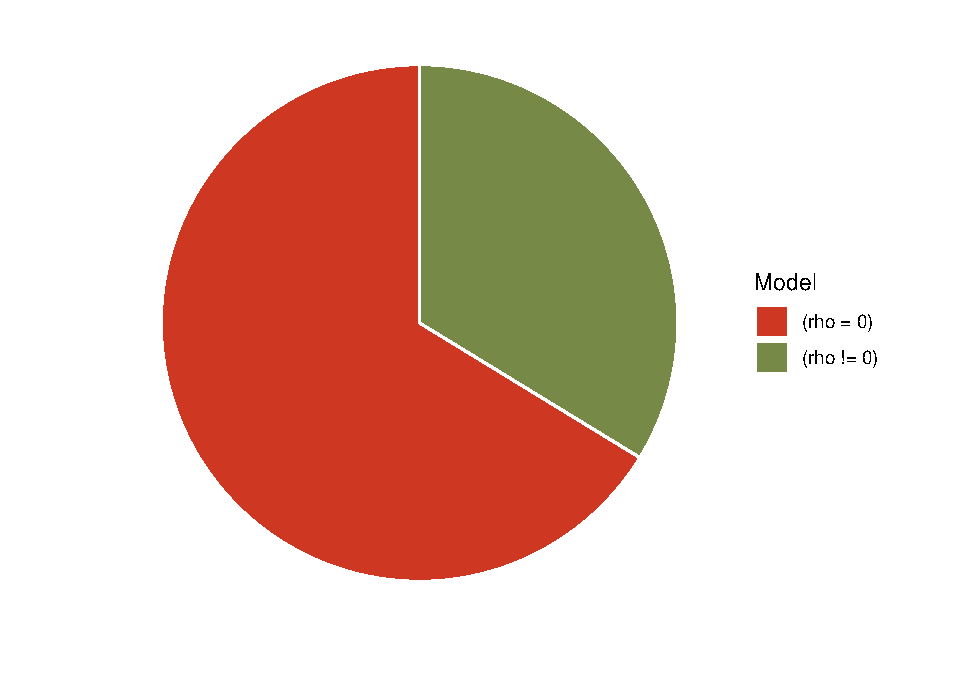
\includegraphics[width=1\linewidth]{paper_files/figure-latex/unnamed-chunk-35-1}

So, after seeing this pizza, how much would you be surprised by the
outcome of a blinded poke?

\hypertarget{t-tests}{%
\subsection{\texorpdfstring{\emph{t}-tests}{t-tests}}\label{t-tests}}

\hypertarget{versicolor-vs.-virginica}{%
\subsubsection{Versicolor
vs.~virginica}\label{versicolor-vs.-virginica}}

Bayesian \emph{t}-tests can be performed in a very similar way to
correlations. As we are particularly interested in two levels of the
\texttt{Species} factor, \emph{versicolor} and \emph{virginica}. We will
start by filtering out from \texttt{iris} the non-relevant observations
corresponding to the \emph{setosa} specie, and we will then visualise
the observations and the distribution of the \texttt{Sepal.Width}
variable.

\begin{Shaded}
\begin{Highlighting}[]
\FunctionTok{library}\NormalTok{(dplyr)}
\FunctionTok{library}\NormalTok{(ggplot2)}

\CommentTok{\# Select only two relevant species}
\NormalTok{data }\OtherTok{\textless{}{-}}\NormalTok{ iris }\SpecialCharTok{\%\textgreater{}\%}
  \FunctionTok{filter}\NormalTok{(Species }\SpecialCharTok{!=} \StringTok{"setosa"}\NormalTok{) }\SpecialCharTok{\%\textgreater{}\%}
  \FunctionTok{droplevels}\NormalTok{()}

\CommentTok{\# Visualise distributions and observations}
\NormalTok{data }\SpecialCharTok{\%\textgreater{}\%}
  \FunctionTok{ggplot}\NormalTok{(}\FunctionTok{aes}\NormalTok{(}\AttributeTok{x =}\NormalTok{ Species, }\AttributeTok{y =}\NormalTok{ Sepal.Width, }\AttributeTok{fill =}\NormalTok{ Species)) }\SpecialCharTok{+}
  \FunctionTok{geom\_violindot}\NormalTok{(}\AttributeTok{fill\_dots =} \StringTok{"black"}\NormalTok{, }\AttributeTok{size\_dots =} \DecValTok{1}\NormalTok{) }\SpecialCharTok{+}
  \FunctionTok{scale\_fill\_material}\NormalTok{() }\SpecialCharTok{+}
  \FunctionTok{theme\_modern}\NormalTok{()}
\end{Highlighting}
\end{Shaded}

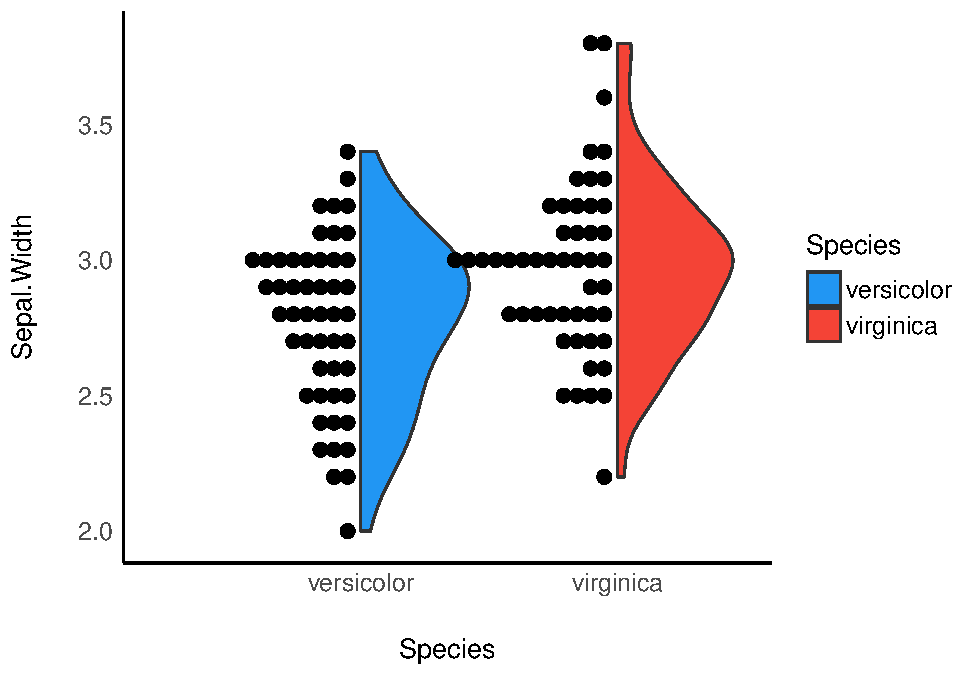
\includegraphics[width=1\linewidth]{paper_files/figure-latex/unnamed-chunk-36-1}

It \emph{seems} (visually) that \emph{virgnica} flowers have, on
average, a slightly higer width of sepals. Let's assess this difference
statistically by using the \texttt{ttestBF()} function in the
\texttt{BayesFactor} package.

\hypertarget{compute-the-bayesian-t-test}{%
\subsubsection{\texorpdfstring{Compute the Bayesian
\emph{t}-test}{Compute the Bayesian t-test}}\label{compute-the-bayesian-t-test}}

\begin{Shaded}
\begin{Highlighting}[]
\NormalTok{result }\OtherTok{\textless{}{-}}\NormalTok{ BayesFactor}\SpecialCharTok{::}\FunctionTok{ttestBF}\NormalTok{(}\AttributeTok{formula =}\NormalTok{ Sepal.Width }\SpecialCharTok{\textasciitilde{}}\NormalTok{ Species, }\AttributeTok{data =}\NormalTok{ data)}
\FunctionTok{describe\_posterior}\NormalTok{(result)}
\CommentTok{\#\textgreater{} Summary of Posterior Distribution}
\CommentTok{\#\textgreater{} }
\CommentTok{\#\textgreater{} Parameter  | Median |       95\% CI |     pd |          ROPE | \% in ROPE |    BF |              Prior}
\CommentTok{\#\textgreater{} {-}{-}{-}{-}{-}{-}{-}{-}{-}{-}{-}{-}{-}{-}{-}{-}{-}{-}{-}{-}{-}{-}{-}{-}{-}{-}{-}{-}{-}{-}{-}{-}{-}{-}{-}{-}{-}{-}{-}{-}{-}{-}{-}{-}{-}{-}{-}{-}{-}{-}{-}{-}{-}{-}{-}{-}{-}{-}{-}{-}{-}{-}{-}{-}{-}{-}{-}{-}{-}{-}{-}{-}{-}{-}{-}{-}{-}{-}{-}{-}{-}{-}{-}{-}{-}{-}{-}{-}{-}{-}{-}{-}{-}{-}{-}{-}{-}{-}{-}{-}}
\CommentTok{\#\textgreater{} Difference |   0.19 | [0.07, 0.31] | 99.90\% | [{-}0.03, 0.03] |        0\% | 17.72 | Cauchy (0 +{-} 0.71)}
\end{Highlighting}
\end{Shaded}

From the indices, we can say that the difference of \texttt{Sepal.Width}
between \emph{virginica} and \emph{versicolor} has a probability of
100\% of being negative {[}\emph{from the pd and the sign of the
median}{]} (median = -0.19, 89\% CI {[}-0.29, -0.092{]}). The data
provides a strong evidence against the null hypothesis (BF = 18).

Keep that in mind as we will see another way of investigating this
question.

\hypertarget{logistic-model}{%
\subsection{Logistic Model}\label{logistic-model}}

A hypothesis for which one uses a \emph{t}-test can also be tested using
a binomial model (\emph{e.g.}, a logistic model). Indeed, it is possible
to reformulate the following hypothesis, ``there is an important
difference in this variable between the two groups'' with the hypothesis
``this variable is able to discriminate between (or classify) the two
groups.'' However, these models are much more powerful than a
\emph{t}-test.

In the case of the difference of \texttt{Sepal.Width} between
\emph{virginica} and \emph{versicolor}, the question becomes, how well
can we classify the two species using only \texttt{Sepal.Width}.

\hypertarget{fit-the-model}{%
\subsubsection{Fit the model}\label{fit-the-model}}

\begin{Shaded}
\begin{Highlighting}[]
\FunctionTok{library}\NormalTok{(rstanarm)}

\NormalTok{model }\OtherTok{\textless{}{-}} \FunctionTok{stan\_glm}\NormalTok{(}
\NormalTok{    Species }\SpecialCharTok{\textasciitilde{}}\NormalTok{ Sepal.Width,}
    \AttributeTok{data =}\NormalTok{ data,}
    \AttributeTok{family =} \StringTok{"binomial"}\NormalTok{,}
    \AttributeTok{refresh =} \DecValTok{0}
\NormalTok{  )}
\end{Highlighting}
\end{Shaded}

\hypertarget{visualise-the-model}{%
\subsubsection{Visualise the model}\label{visualise-the-model}}

Using the
\href{https://github.com/easystats/modelbased}{\texttt{modelbased}}
package.

\begin{Shaded}
\begin{Highlighting}[]
\FunctionTok{library}\NormalTok{(modelbased)}

\NormalTok{vizdata }\OtherTok{\textless{}{-}} \FunctionTok{estimate\_relation}\NormalTok{(model)}

\FunctionTok{ggplot}\NormalTok{(vizdata, }\FunctionTok{aes}\NormalTok{(}\AttributeTok{x =}\NormalTok{ Sepal.Width, }\AttributeTok{y =}\NormalTok{ Predicted)) }\SpecialCharTok{+}
  \FunctionTok{geom\_ribbon}\NormalTok{(}\FunctionTok{aes}\NormalTok{(}\AttributeTok{ymin =}\NormalTok{ CI\_low, }\AttributeTok{ymax =}\NormalTok{ CI\_high), }\AttributeTok{alpha =} \FloatTok{0.5}\NormalTok{) }\SpecialCharTok{+}
  \FunctionTok{geom\_line}\NormalTok{() }\SpecialCharTok{+} 
  \FunctionTok{ylab}\NormalTok{(}\StringTok{"Probability of being virginica"}\NormalTok{) }\SpecialCharTok{+}
  \FunctionTok{theme\_modern}\NormalTok{()}
\end{Highlighting}
\end{Shaded}

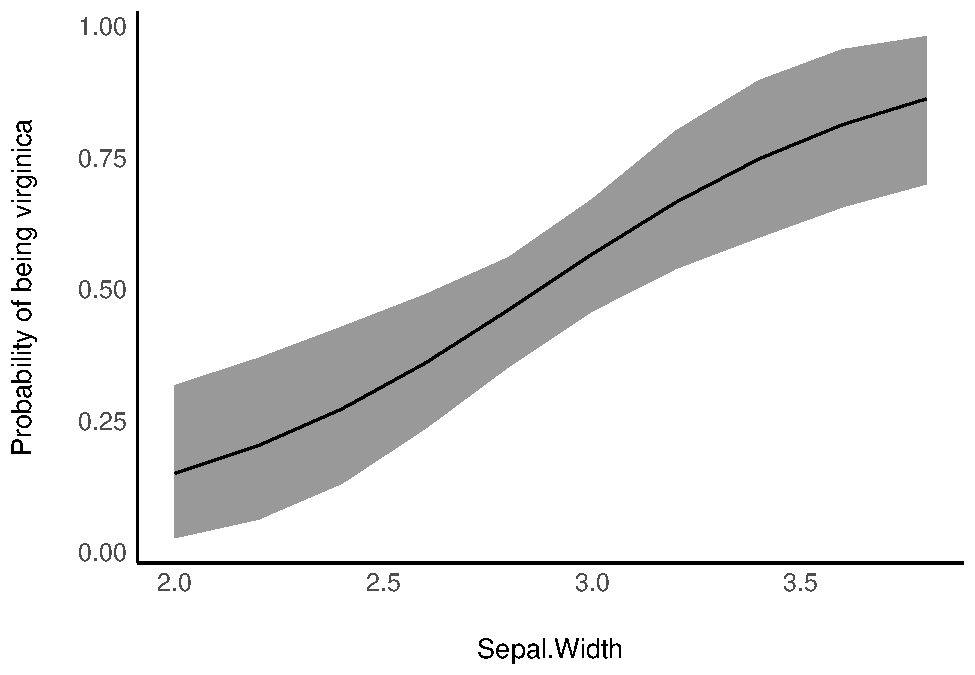
\includegraphics[width=1\linewidth]{paper_files/figure-latex/unnamed-chunk-39-1}

\hypertarget{performance-and-parameters}{%
\subsubsection{Performance and
Parameters}\label{performance-and-parameters}}

Once again, we can extract all indices of interest for the posterior
distribution using our old pal \texttt{describe\_posterior()}.

\begin{Shaded}
\begin{Highlighting}[]
\FunctionTok{describe\_posterior}\NormalTok{(model, }\AttributeTok{test =} \FunctionTok{c}\NormalTok{(}\StringTok{"pd"}\NormalTok{, }\StringTok{"ROPE"}\NormalTok{, }\StringTok{"BF"}\NormalTok{))}
\CommentTok{\#\textgreater{} Summary of Posterior Distribution}
\CommentTok{\#\textgreater{} }
\CommentTok{\#\textgreater{} Parameter   | Median |          95\% CI |     pd |          ROPE | \% in ROPE |  Rhat |     ESS |    BF}
\CommentTok{\#\textgreater{} {-}{-}{-}{-}{-}{-}{-}{-}{-}{-}{-}{-}{-}{-}{-}{-}{-}{-}{-}{-}{-}{-}{-}{-}{-}{-}{-}{-}{-}{-}{-}{-}{-}{-}{-}{-}{-}{-}{-}{-}{-}{-}{-}{-}{-}{-}{-}{-}{-}{-}{-}{-}{-}{-}{-}{-}{-}{-}{-}{-}{-}{-}{-}{-}{-}{-}{-}{-}{-}{-}{-}{-}{-}{-}{-}{-}{-}{-}{-}{-}{-}{-}{-}{-}{-}{-}{-}{-}{-}{-}{-}{-}{-}{-}{-}{-}{-}{-}{-}{-}{-}}
\CommentTok{\#\textgreater{} (Intercept) |  {-}6.13 | [{-}10.27, {-}2.15] | 99.95\% | [{-}0.18, 0.18] |        0\% | 1.000 | 2286.00 | 17.33}
\CommentTok{\#\textgreater{} Sepal.Width |   2.13 | [  0.76,  3.60] | 99.98\% | [{-}0.18, 0.18] |        0\% | 1.000 | 2323.00 | 17.39}
\end{Highlighting}
\end{Shaded}

\begin{Shaded}
\begin{Highlighting}[]
\FunctionTok{library}\NormalTok{(performance)}

\FunctionTok{model\_performance}\NormalTok{(model)}
\CommentTok{\#\textgreater{} \# Indices of model performance}
\CommentTok{\#\textgreater{} }
\CommentTok{\#\textgreater{} ELPD    | ELPD\_SE |   LOOIC | LOOIC\_SE |    WAIC |    R2 |  RMSE | Sigma | Log\_loss | Score\_log | Score\_spherical}
\CommentTok{\#\textgreater{} {-}{-}{-}{-}{-}{-}{-}{-}{-}{-}{-}{-}{-}{-}{-}{-}{-}{-}{-}{-}{-}{-}{-}{-}{-}{-}{-}{-}{-}{-}{-}{-}{-}{-}{-}{-}{-}{-}{-}{-}{-}{-}{-}{-}{-}{-}{-}{-}{-}{-}{-}{-}{-}{-}{-}{-}{-}{-}{-}{-}{-}{-}{-}{-}{-}{-}{-}{-}{-}{-}{-}{-}{-}{-}{-}{-}{-}{-}{-}{-}{-}{-}{-}{-}{-}{-}{-}{-}{-}{-}{-}{-}{-}{-}{-}{-}{-}{-}{-}{-}{-}{-}{-}{-}{-}{-}{-}{-}{-}{-}{-}{-}{-}}
\CommentTok{\#\textgreater{} {-}66.257 |   3.044 | 132.514 |    6.089 | 132.505 | 0.098 | 0.477 | 1.000 |    0.643 |   {-}34.992 |           0.014}
\end{Highlighting}
\end{Shaded}

\hypertarget{visualise-the-indices}{%
\subsubsection{Visualise the indices}\label{visualise-the-indices}}

TO DO.

\begin{Shaded}
\begin{Highlighting}[]
\FunctionTok{library}\NormalTok{(see)}

\FunctionTok{plot}\NormalTok{(}\FunctionTok{rope}\NormalTok{(result))}
\end{Highlighting}
\end{Shaded}

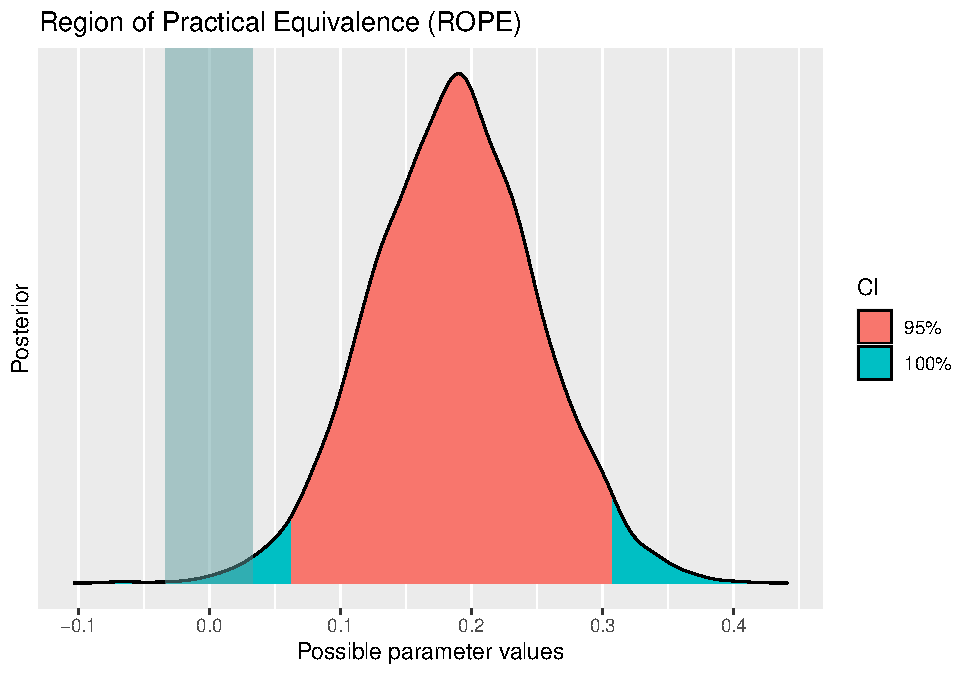
\includegraphics[width=1\linewidth]{paper_files/figure-latex/unnamed-chunk-42-1}

\hypertarget{diagnostic-indices}{%
\subsubsection{Diagnostic Indices}\label{diagnostic-indices}}

About diagnostic indices such as Rhat and ESS.

\hypertarget{acknowledgments}{%
\section{Acknowledgments}\label{acknowledgments}}

\emph{see} is part of the collaborative
\href{https://github.com/easystats/easystats}{\emph{easystats}}
ecosystem. Thus, we thank the
\href{https://github.com/orgs/easystats/people}{members of easystats} as
well as the users.

\hypertarget{references}{%
\section*{References}\label{references}}
\addcontentsline{toc}{section}{References}

\hypertarget{refs}{}
\begin{CSLReferences}{1}{0}
\leavevmode\hypertarget{ref-andrews2013prior}{}%
Andrews, M., \& Baguley, T. (2013). Prior approval: The growth of
bayesian methods in psychology. \emph{British Journal of Mathematical
and Statistical Psychology}, \emph{66}(1), 1--7.

\leavevmode\hypertarget{ref-benjamin2018redefine}{}%
Benjamin, D. J., Berger, J. O., Johannesson, M., Nosek, B. A.,
Wagenmakers, E.-J., Berk, R., \ldots{} others. (2018). Redefine
statistical significance. \emph{Nature Human Behaviour}, \emph{2}(1), 6.

\leavevmode\hypertarget{ref-chambers2014instead}{}%
Chambers, C. D., Feredoes, E., Muthukumaraswamy, S. D., \& Etchells, P.
(2014). Instead of 'playing the game' it is time to change the rules:
Registered reports at AIMS neuroscience and beyond. \emph{AIMS
Neuroscience}, \emph{1}(1), 4--17.

\leavevmode\hypertarget{ref-cohen1988statistical}{}%
Cohen, J. (1988). \emph{Statistical power analysis for the social
sciences}.

\leavevmode\hypertarget{ref-etz2016bayesian}{}%
Etz, A., \& Vandekerckhove, J. (2016). A bayesian perspective on the
reproducibility project: psychology. \emph{PloS One}, \emph{11}(2),
e0149794.

\leavevmode\hypertarget{ref-kruschke2014doing}{}%
Kruschke, J. (2014). \emph{Doing bayesian data analysis: A tutorial with
r, JAGS, and stan}. Academic Press.

\leavevmode\hypertarget{ref-kruschke2010believe}{}%
Kruschke, J. K. (2010). What to believe: Bayesian methods for data
analysis. \emph{Trends in Cognitive Sciences}, \emph{14}(7), 293--300.

\leavevmode\hypertarget{ref-kruschke2012time}{}%
Kruschke, J. K., Aguinis, H., \& Joo, H. (2012). The time has come:
Bayesian methods for data analysis in the organizational sciences.
\emph{Organizational Research Methods}, \emph{15}(4), 722--752.

\leavevmode\hypertarget{ref-mcelreath2018statistical}{}%
McElreath, R. (2018). \emph{Statistical rethinking: A bayesian course
with examples in r and stan}. Chapman; Hall/CRC.

\leavevmode\hypertarget{ref-szucs2016empirical}{}%
Szucs, D., \& Ioannidis, J. P. (2016). Empirical assessment of published
effect sizes and power in the recent cognitive neuroscience and
psychology literature. \emph{BioRxiv}, 071530.

\leavevmode\hypertarget{ref-wagenmakers2018bayesian}{}%
Wagenmakers, E.-J., Marsman, M., Jamil, T., Ly, A., Verhagen, J., Love,
J., \ldots{} others. (2018). Bayesian inference for psychology. Part i:
Theoretical advantages and practical ramifications. \emph{Psychonomic
Bulletin \& Review}, \emph{25}(1), 35--57.

\end{CSLReferences}

\end{document}
